% !TEX root = main.tex
\RequirePackage[l2tabu, orthodox]{nag} %if this document is out-dated
\documentclass[twoside,12pt,openright]{book}
\RequirePackage{longtable}   % 附录表格跨页（须在 liTemElegX 加载 arydshln 之前）
\usepackage[
    geometry,
    fancy,
    font,
    color,
    graphicx,
    table,
    math,
    phys,
    chem,
    env
]{liTemElegXv2.4}
\usepackage{LuaTemElegX}    % LuaLaTeX（LuaHBTeX）字体配置，替代 xeTemElegX/pTemElegX
\usepackage{TemElegXref}
\usepackage{xltabular}   % 附录 tabularx 型表格跨页
\usepackage{rotating}    % 附录 A 周期表横向图旋转占满竖向 A4
\usepackage{pdflscape}   % 附录 A 周期表横向整页
% \usepackage{pdfpages}  % 附录 A（元素周期表）插入 PDF 时启用，参见 appendix/appendix-periodic.tex
% \graphicspath{{../Pic/}{../figures/}{../images/}}
% \raggedbottom
\hypersetup{ %
    pdftitle = {} , % PDFのタイトル
    pdfauthor = {} , % PDFの作成者
    pdfsubject = {上海市进才中学化学笔记},    % 主題
    pdfkeywords = {Chemistry, notes, senior middle school, Shanghai},  %関鍵詞
    pdfcreator  = {LuaHBTeX with hyperref},    %工具
    pdflang = {zh}
}
\setcounter{secnumdepth}{3}  % 让 subsubsection 有编号
\setcounter{tocdepth}{2}        % 目录只显示到 subsection
\hypersetup{bookmarksdepth=3}   % PDF 书签显示到 subsubsection

\newcommand{\cemh}[1]{\!\,\ce{#1}\,\!}
\newcommand{\xleq}[2][\hspace{5mm}]{\,\!\,\ensuremath{\xlongequal[\text{#1}]{\text{#2}}}\,\!\,}
\newcommand{\conc}[2][c]{\ensuremath{#1(\cemh{#2})}}
\newcommand{\cmark}{{\ssans\char"2713}}  % ✓ CHECK MARK
\newcommand{\xmark}{{\ssans\char"2717}}  % ✗ BALLOT X
\newcommand{\hcmark}{{\ssans\char"2714}} % ✔ HEAVY CHECK MARK
\newcommand{\hxmark}{{\ssans\char"2718}} % ✘ HEAVY BALLOT X

% 附录数据清单：逐条独立数据，需适度行距（\setlist{nosep} 全局压平后在此恢复）
\newlist{datas}{itemize}{2}
\setlist[datas]{label=\textbullet, leftmargin=1em, itemsep=2pt, topsep=3pt, parsep=0pt}


\title{化学笔记}
\author{}
\date{\today}

\makeatletter
\def\@endpart{\par\nobreak\vfil\newpage}
\makeatother
\includeonly{chapters/2501,chapters/2502}

\begin{document}
    \maketitle
    \tableofcontents

    \cleardoublepage
    \part{二〇二五学年第一学期}

    本学期在 \nameref{chap:水溶液中的平衡} 体系中具体补充建立化学平衡的完整认知框架。首先在 \nameref{sect:3.0基础知识复习} 中复习电解质与非电解质、强弱电解质等基本概念（\nameref{tab:弱酸-课本3.3} 列举了常见弱酸弱碱的电离平衡常数数据），在此基础上进入 \nameref{sect:水的电离和溶液酸碱性}，认识水的电离平衡与溶液的酸碱性，引入水的离子积 \(K_\text{W}\) 与 pH 的计算体系（包括 \nameref{subsec:测量pH的方法}、\nameref{subsec:有关pH的计算} 和 \nameref{subsec:水电离出的[H+]和[OH^-]}）。随后进入 \nameref{sect:弱电解质的电离平衡}，建立 \nameref{subsec:电离度} \(\alpha\) 与 \nameref{subsec:电离常数} \(K_\text{i}\) 的定量分析方法，并结合近似处理与计算技巧，培养解决实际问题的能力。进而探讨 \nameref{sect:盐类水解} 的 \nameref{subsec:盐类水解的原理}、\nameref{subsec:盐类水解的规律} 与 \nameref{subsubsec:水解常数}，加深对溶液中微粒行为的理解，并设 \nameref{sect:专题——溶液中的微粒浓度比较} 系统归纳溶液中微粒浓度比较的三大守恒方法。转而进入 \nameref{sect:酸碱滴定} 的实践操作，涵盖 \nameref{subsec:中和滴定的原理}、\nameref{subsec:实验仪器}（\nameref{subsubsec:滴定管}）、\nameref{subsec:滴定过程} 与 \nameref{subsec:指示剂选择与滴定过程中的颜色变化}（参见 \nameref{fig:titration_indicators_2501}），并拓展至 \nameref{subsec:滴定典型案例分析} 与 \nameref{subsec:拓展：氧化还原滴定}（\nameref{subsubsec:高锰酸钾法氧化还原滴定}、\nameref{subsubsec:碘量法氧化还原滴定}），强调实验设计与结果解读。此后讨论 \nameref{sect:沉淀溶解平衡}，以 \nameref{subsec:溶度积常数}（\nameref{subsubsec:Ksp意义和影响因素}、\nameref{subsubsec:溶度积规则}）为核心，分析 \nameref{subsec:沉淀溶解平衡的移动}（\nameref{subsubsec:沉淀的转化}、\nameref{subsubsec:沉淀的溶解}），进而理解共离子效应、络合反应与沉淀溶解在实际问题中的应用。
    
    在溶液平衡体系之外，还涉及有机化合物的结构基础，并深入分子层面，运用 \nameref{sect:VSEPR和杂化轨道理论}（\nameref{subsec:VSEPR}、\nameref{subsec:杂化轨道理论}、\nameref{subsec:等电子体原理}）解释分子的空间构型。结合官能团与同分异构体，在 \nameref{sect:分子结构与物质性质} 中分析有机分子的性质与反应趋势，进而探讨 \nameref{subsec:分子极性}、\nameref{subsec:范德华力} 与 \nameref{subsec:氢键}（含 \nameref{subsubsec:氢键对物质性质的影响}）对物质性质的影响，以及 \nameref{subsec:相似相溶原理}。通过实例加深对分子间作用力与物理性质关系的理解，为后续有机化学与物质结构的学习奠定基础。

    \cleardoublepage
    \chapter{水溶液中的平衡} \label{chap:水溶液中的平衡}

\setcounter{section}{-1}
\section{\S 3.0 基础知识复习}\label{sect:3.0基础知识复习}

    \subsection{电解质与非电解质} \label{subsec:电解质与非电解质}

        在水溶液\uline{或}熔融状态下\(\overset{\text{\textcolor{blue}{电离}}}{\text{导电}}\)的\uline{化合物}叫做电解质；
        
        在水溶液\uline{和}熔融状态下都不能\(\overset{\text{\textcolor{blue}{电离}}}{\text{导电}}\)的\uline{化合物}叫做非电解质。

        \textcolor{red}{必须是化合物本身电离，而非与水反应后产生离子}

        \textcolor{red}{是物质具有的性质，与物质所处状态无关}

        \textcolor{blue}{{\bfseries 电解质}：酸、碱、盐、水}

        \textcolor{blue}{电解质导电原因：有\uline{自由移动}的离子}

        \qquad 电离：电解质产生自由移动离子的过程

        \textcolor{red}{\(\therefore\text{溶液的导电能力}\propto\text{离子浓度}\)}

        离子浓度\(\left\{\begin{matrix}
            \text{溶液浓度}\\
            \text{电离程度}
        \end{matrix}\right.\)

    \subsection{强弱电解质}\label{subsec:强弱电解质}

        强电解质——在水溶液中\textcolor{blue}{完全电离}为离子的电解质
        
        \phantom{强电解质——}电离方程式用``\cemh{\xleq{}}''\quad 只存在离子

        弱电解质——在水溶液中\textcolor{blue}{部分电离}为离子的电解质
        
        \phantom{强电解质——}电离方程式用``\cemh{<=>}''\quad 离子、分子都有

        强电解质：强酸、强碱、绝大多数盐

        弱电解质：弱酸、弱碱、水

        \begin{itemize}
            \item 常见强酸：\cemh{H2SO4}、\cemh{HNO3}、\cemh{HCl}、\cemh{HBr}、\cemh{HI}、\cemh{HClO4}
            \item 常见强碱：\cemh{KOH}、\cemh{NaOH}、\cemh{Ba(OH)2}、\cemh{Ca(OH)2}
            \item 常见弱酸：见 \textbf{表~\ref{tab:弱酸-课本3.3}}
            \item 常见弱碱：氨水、不溶性碱
        \end{itemize}

        \begin{table}[htbp]
            \centering
            \caption{常见弱酸、弱碱的电离平衡常数（\SI{25}{\degreeCelsius}）}
            \label{tab:弱酸-课本3.3}
            \begin{tabular}{|c|c||c|c|}
                \toprule
                \small 一元弱酸{\footnotesize 或}弱碱 &\small \( K_\text{a} \) {\footnotesize 或} \( K_\text{b} \) &\small 多元弱酸 &\small \( K_\text{a1} \) {\footnotesize 和} \( K_\text{a2} \) \\
                \midrule\footnotesize
                \cemh{HCOOH}\footnotemark &\footnotesize \SI{1.8E-4}{} &\footnotesize 
                \multirow{2}[0]{*}{\cemh{H2CO3}} &\footnotesize \( K_\text{a1} = \SI{4.2E-7}{} \) \\\footnotesize
                \cemh{HNO2} &\footnotesize \SI{7.2E-4}{} &\footnotesize 
                                                    &\footnotesize \( K_\text{a2} = \SI{4.8E-11}{} \) \\\footnotesize 
                \cemh{HF} &\footnotesize \SI{5.6E-4}{} &\footnotesize 
                \multirow{2}[0]{*}{\cemh{H2SO3}} &\footnotesize \( K_\text{a1} = \SI{1.2E-2}{} \) \\\footnotesize
                \cemh{CH3COOH} &\footnotesize \SI{1.8E-5}{} &\footnotesize 
                                                    &\footnotesize \( K_\text{a2} = \SI{6.2E-8}{} \) \\\footnotesize
                \cemh{HCN}\footnotemark &\footnotesize \SI{4.0E-10}{} &\footnotesize 
                \multirow{2}[0]{*}{\chemfig{COOH(-[2, .7]COOH)}}\footnotemark &\footnotesize \( K_\text{a1} = \SI{5.6E-2}{} \) \\\footnotesize 
                \cemh{NH3 . H2O} &\footnotesize \SI{1.8E-5}{} &\footnotesize 
                                                                                &\footnotesize \( K_\text{a2} = \SI{5.4E-5}{} \) \\
                \midrule\footnotesize
                \multirow{2}[0]{*}{\cemh{H2S}} &\footnotesize \( K_\text{a1} = \SI{5.7E-8}{} \) &\footnotesize 
                \multirow{3}[0]{*}{\cemh{H3PO4}} &\footnotesize \( K_\text{a1} = \SI{7.52E-3}{} \)  \\\footnotesize
                                                &\footnotesize \( K_\text{a2} = \SI{1.2E-15}{} \) &\footnotesize 
                                                    &\footnotesize \( K_\text{a2} = \SI{6.23E-8}{} \) \\\footnotesize
                                                &&&\footnotesize \( K_\text{a3} = \SI{2.2E-13}{} \) \\
                \bottomrule
            \end{tabular}
        \end{table}
        \footnotetext[1]{甲酸}\footnotetext[2]{氢氰酸}\footnotetext[3]{草酸}
    
    \subsection{电解质与离子、共价化合物的关系}\label{subsec:电解质与离子、共价化合物的关系}

        离子化合物——强电解质

        共价化合物\(\left\{\begin{matrix}
            \text{强极性键\hspace{1em}} & \text{——强酸——} & \text{强电解质}\\
            \text{较强极性键} & \text{——\phantom{强酸}——} & \text{弱电解质}\\
            \text{弱极性键\hspace{1em}} & \text{——\phantom{强酸}——} & \text{非电解质}
        \end{matrix}\right.\)

        离子化合物——水溶液、熔融状态电离

        共价化合物——熔融状态电离
    

\section{\S 3.1 水的电离和溶液酸碱性}\label{sect:水的电离和溶液酸碱性}

    \subsection{水的电离}\label{subsec:水的电离}
        
        \cemh{H2O + H2O <=> H2O+ + OH^-}，
        简写为 \cemh{H2O <=> H+ + OH^-}

        \textcolor{red}{往纯水里加入酸或碱，水的电离平衡如何移动？}

        \textcolor{red}{\(c(\cemh{H+})\)与\(c(\cemh{OH^-})\)如何变化？}

        水溶液中\(c(\cemh{H+})\)与\(c(\cemh{OH^-})\)\textcolor{red}{此消彼长}

        一定温度下，纯水或稀溶液中：\(K_\text{W} = \cemh{[H+]} \cdot \cemh{[OH^-]}\)
        \footnote{\cemh{[H2O]} 在稀溶液/纯水中近似为常数}

        \(K_\text{W}\)——水的离子积常数\qquad 简称：水的离子积

        \SI{25}{\degreeCelsius}时： \( K_\text{W} = \SI{1E-14}{}\)\quad\qquad \textcolor{red}{\( K_\text{W} \) 随温度如何变化？}

        \SI{99}{\degreeCelsius}时： \( K_\text{W} = \SI{1E-12}{}\)\quad\qquad \textcolor{blue}{温度变化不大时，使用\SI{25}{\degreeCelsius}时的\( K_\text{W} \)}

    \subsection{溶液酸碱性与\texorpdfstring{\cemh{[H+]}}{H⁺}、\texorpdfstring{\cemh{[OH^-]}}{OH⁻}及 pH 的关系}\label{subsec:溶液酸碱性与[H+]、[OH^-]及pH的关系}

        \( \cemh{pH} = -\lg{}\cemh{[H+]} \) 

        \noindent
        \begin{tabular}{ccccc}
                        & 任何条件下 & & 常温下（ \( K_\text{W} = \SI{1E-14}{}\) ）\\
            中性溶液 & \( \cemh{[H+]} = \cemh{[OH^-]} \) & \( \cemh{pH} = 7 \) & \textcolor{blue}{\( \cemh{[H+]} = \cemh{[OH^-]} = \SI{1E-7}{\mole\per\litre} \) } \\
            酸性溶液 & \( \cemh{[H+]} > \cemh{[OH^-]} \) & \( \cemh{pH} < 7 \) & \textcolor{blue}{\( \cemh{[H+]} > \SI{1E-7}{\mole\per\litre} > \cemh{[OH^-]} \) } \\
            碱性溶液 & \( \cemh{[H+]} < \cemh{[OH^-]} \) & \( \cemh{pH} > 7 \) & \textcolor{blue}{\( \cemh{[H+]} < \SI{1E-7}{\mole\per\litre} < \cemh{[OH^-]} \) }
        \end{tabular}

        \textcolor{blue}{\cemh{[H+]} 越大，溶液酸性越强；\cemh{[H+]} 越小，溶液酸性越弱；}

        \textcolor{blue}{\cemh{[OH^-]} 越大，溶液碱性越强；\cemh{[OH^-]} 越小，溶液碱性越弱。}

        \textcolor{blue}{pH 越小，\cemh{[H+]} 越大，\cemh{[OH^-]} 越小，溶液酸性越强，碱性越弱；}

        \textcolor{blue}{pH 越大，\cemh{[H+]} 越小，\cemh{[OH^-]} 越大，溶液酸性越弱，碱性越强。}

        pH 的适用范围：\numrange{0}{14}

    \subsection{测量 pH 的方法}\label{subsec:测量pH的方法}
        \subsubsection{酸碱指示剂}\label{subsubsec:酸碱指示剂}

            指示剂的变色范围：

            \begingroup
            \setlength{\fboxsep}{0pt}
            % \small
            \newcommand{\boxstrut}{\rule[-0.2em]{0pt}{1.2em}}
            \begin{center}
            \begin{tabular}{lll}
                甲基橙 &\small 1\colorbox{red}{\makebox[4.2em]{\boxstrut 红色}}\colorbox{orange}{\makebox[2.6em]{\boxstrut 橙色}}\colorbox{yellow}{\makebox[15.2em]{\boxstrut 黄色}}12 & --3.1--4.4-- \\
                甲基红 &\small 1\colorbox{red}{\makebox[6.8em]{\boxstrut 红色}}\colorbox{orange}{\makebox[3.6em]{\boxstrut 橙色}}\colorbox{yellow}{\makebox[11.6em]{\boxstrut 黄色}}12 & --4.4--6.2-- \\
                石蕊   &\small 1\colorbox{red}{\makebox[7em]{\boxstrut 红色}}\colorbox{violet!85!white}{\makebox[7.6em]{\boxstrut \color{white}紫色}}\colorbox{blue}{\makebox[7.4em]{\boxstrut \color{white}蓝色}}12 & --4.5--8.3-- \\
                酚酞   &\small 1\colorbox{gray!25!white}{\makebox[14em]{\boxstrut 无色}}\colorbox{red!50!white}{\makebox[4em]{\boxstrut 粉红色}}\colorbox{red}{\makebox[4em]{\boxstrut 红色}}12 & --8.0--10.0-- \\
            \end{tabular}
            \end{center}
            \endgroup

        \subsubsection{pH 试纸}\label{subsubsec:pH试纸}

            广泛 pH 试纸（普通 pH 试纸）：只能测出\numrange{1}{14}范围的整数值

            精密 pH 试纸（有适用范围，读数精确到 \( 0.1 \) ）

            pH 试纸的使用注意事项——不可润湿

        \subsubsection{pH 计（酸度计）}\label{subsubsec:pH计}
            \textcolor{red}{测定前用蒸馏水洗净探头}

            直接读数，精确到 \( 0.01 \)

    \subsection{有关 pH 的计算}\label{subsec:有关pH的计算}

        \subsubsection{\texorpdfstring{\cemh{[H+]}}{H⁺}与 pH 之间的换算}\label{subsubsec:[H+]与pH之间的换算}
            \begin{xmp}
                [pH 计算例一]
                {}
                []
                []
                \vspace{-\baselineskip}
                \begin{enumerate}[itemindent=0em]
                    \item 已知\(c(\cemh{Cl-}) = \SI{0.01}{\mole\per\litre}\)，
                求其\(\cemh{pH}=\)\uline{\makebox[1.5em]{2}}，\(\cemh{[OH^-]}=\)\newline\uline{\makebox[9em]{\SI{1E-12}{\mole\per\litre}}}；
                    \item \(\cemh{pH} = 3\) 的稀硫酸的溶液浓度为\uline{\makebox[4.5em]{\SI{5E-4}{}}}\SI{}{\mole\per\litre}。
                \end{enumerate}
            \end{xmp}
            \begin{xmp}
                [pH 计算例二]
                {}
                []
                []
                \vspace{-\baselineskip}
                \begin{enumerate}
                    \item \SI{50}{\ml} \(\cemh{pH} = 1\)的盐酸溶液中，\( \conc[n]{H+} =\uline{\makebox[6em]{\SI{0.005}{\mole}}}\)；
                    \item 甲溶液的\(\cemh{pH} = 2\)，乙溶液的\(\cemh{pH} = 5\)，则溶液中 \cemh{[H+]} 甲是乙的\uline{\makebox[4em]{1000}}倍，\cemh{[OH^-]} 甲是乙的\uline{\makebox[4em]{\(\frac{1}{1000}\)}}倍。
                \end{enumerate}
            \end{xmp}
            
        \subsubsection{\texorpdfstring{\cemh{[OH^-]}}{OH⁻}与 pH 之间的换算}\label{subsubsec:[OH^-]与pH之间的换算}
            \begin{xmp}
                [pH 计算例三]
                {}
                []
                []
                \vspace{-\baselineskip}
                \begin{enumerate}
                    \item \SI{0.05}{\mole\per\litre}的氢氧化钡溶液，\(\cemh{pH}=\uline{\makebox[1.5em]{13}}\)；
                    \item 配置\(\cemh{pH} = 14\)的 \cemh{NaOH} 溶液\SI{100}{\ml}，需 \cemh{NaOH}\uline{\makebox[1.5em]{2}}\SI{}{\gram}；
                    \item \SI{5.6}{\gram}\,\cemh{KOH} 溶于水配成\SI{1}{\litre}溶液，\(\cemh{[OH^-]}=\uline{\makebox[5.5em]{\SI{0.1}{\mole\per\litre}}}\)，\(\cemh{pH}=\uline{\makebox[1.3em]{13}}\) 。
                \end{enumerate}
            \end{xmp}
            
        \subsubsection{稀释计算}\label{subsubsec:稀释计算}
            \begin{xmp}
                [pH 计算例四]
                {}
                []
                []
                取\SI{1}{\ml}\,\(\cemh{pH}=2\)的盐酸加水稀释到\SI{100}{\ml}后，该溶液的\(\cemh{pH}=\uline{\makebox[1.5em]{4}}\)；

                取\SI{1}{\ml}\,\(\cemh{pH}=12\)的 \cemh{NaOH} 溶液加水稀释到\SI{100}{\ml}后，该溶液的\(\cemh{pH}=\uline{\makebox[1.5em]{10}}\)。
            \end{xmp}
            \begin{xmp}
                [pH 计算例五]
                {}
                []
                []
                将\(\cemh{pH}=5\)的硫酸稀释\(10\)倍，\(\cemh{pH}=\uline{\makebox[1.5em]{6}}\)；

                将\(\cemh{pH}=5\)的硫酸稀释\(1000\)倍，\(\cemh{pH}=\uline{\makebox[1.5em]{7}}\)。
            \end{xmp}

            \textcolor{red}{[小结]：强酸强碱每稀释 \( 10 \) 倍，\cemh{[H+]}、\cemh{[OH^-]} 变化 \( 10 \) 倍，pH 改变 \( 1 \)；}

            \phantom{[小结]：}\textcolor{red}{但酸不会稀释成碱，碱不会稀释成酸，pH 最终逼近 \( 7 \)。}

        \subsubsection{混合计算}\label{subsubsec:混合计算}

        \noindent   1. 酸酸混合

            \stepcounter{example}%例六缺失
            \begin{xmp}
                [pH 计算例七]
                {}
                []
                []
                \(\cemh{pH}=2\)的盐酸\SI{100}{\ml}与 \(\cemh{pH}=3\)的硫酸\SI{200}{\ml}混合后，\(\cemh{pH}=\uline{\makebox[2em]{2.40}}\)。
            \end{xmp}

        \noindent   2. 碱碱混合

            \begin{xmp}
                [pH 计算例八]
                {}
                []
                []
                \(\cemh{pH}=10\)的 \cemh{Ba(OH)2} 溶液与 \(\cemh{pH}=12\)的 \cemh{NaOH} 溶液等体积混合后，溶液中的\(\cemh{[H+]}=\uline{\makebox[9.5em]{\SI{1.96E-12}{\mole\per\litre}}}\)，\(\cemh{pH}=\uline{\makebox[3em]{11.70}}\) 。
            \end{xmp}

        \noindent   3. 酸碱中和

            \begin{xmp}
                [pH 计算例九]
                {}
                []
                []
                \(\cemh{pH}=3\)的硫酸与 \(\cemh{pH}=10\)的 \cemh{NaOH} 溶液混合，若要混合后的溶液\(\cemh{pH}=7\)（恰好完全中和），则硫酸与 \cemh{NaOH} 溶液的体积比为\uline{\makebox[3em]{1:10}} 。
            \end{xmp}

            \begin{xmp}
                [pH 计算例十]
                {}
                []
                []
                把\SI{100.5}{\ml}\,\SI{0.2}{\mole\per\litre}的 \cemh{NaOH} 溶液加入到\SI{99.5}{\ml}\,\SI{0.1}{\mole\per\litre}的硫酸中，充分反应后所得溶液的\(\cemh{pH}=\uline{\makebox[2em]{11}} \)。
            \end{xmp}

        \noindent   4. 其它反应

            \begin{xmp}
                [pH 计算例十一]
                {}
                []
                []
                \SI{0.01}{\mole\per\litre}的硫酸\SI{5}{\ml}与\SI{0.01}{\mole\per\litre}的 \cemh{BaCl2} 溶液\SI{5}{\ml}混合，充分反应后所得溶液的\(\cemh{pH}=\uline{\makebox[2em]{2}}\)。
            \end{xmp}

            \textcolor{red}{[小结]：若反应不涉及 \cemh{H+}、\cemh{OH^-}，相当于稀释}

        \subsubsection{非常温计算}\label{subsubsec:非常温计算}

            \begin{xmp}
                [pH 计算例十二]
                {}
                []
                []
                某温度下，\cemh{NaCl} 溶液\(\cemh{pH}=6.5\)；则该温度下\(\cemh{pH}=2\)的硫酸与\(\cemh{pH}=\uline{\makebox[2.5em]{11}}\)的 \cemh{NaOH} 溶液等体积混合后恰好完全中和。该温度下\(\cemh{pH}=2\)的硫酸与\(\cemh{pH}=10\)的 \cemh{NaOH} 溶液按体积比\(\uline{\makebox[1.5em]{9}}:\uline{\makebox[3em]{101}}\)，混合后溶液\(\cemh{pH}=9\)。
            \end{xmp}

            \textcolor{red}{[小结]：先算出该温度下的\(K_\text{W}\)，其他计算同前。}
            
    \subsection{水电离出的\texorpdfstring{\cemh{[H+]}}{H⁺}和\texorpdfstring{\cemh{[OH^-]}}{OH⁻}\texorpdfstring{\footnotemark}{}}\label{subsec:水电离出的[H+]和[OH^-]}\footnotetext{暂时只有酸和碱}

        〔常温下〕某溶液中水电离出的\(\cemh{[H+]}=\SI{1E-11}{\mole\per\litre}\)，该溶液\(\cemh{pH}=\uline{\makebox[5em]{3 或 11}}\)；

        〔常温下〕某溶液中水电离出的\(\cemh{[OH^-]}=\SI{1E-11}{\mole\per\litre}\)，该溶液\(\cemh{pH}=\uline{\makebox[5em]{3 或 11}}\)。

        1、pH＝3 的盐酸溶液中，水电离出的\(\cemh{[H+]}_\text{水}=\uline{\makebox[9em]{\SI{1E-12}{\mole\per\litre}}}\)，水电离出的\(\cemh{[OH^-]}_\text{水}=\uline{\makebox[9em]{\SI{1E-12}{\mole\per\litre}}}\) 。

        2、pH＝11 的 \cemh{NaOH} 溶液中，水电离出的\(\cemh{[H+]}_\text{水}=\uline{\makebox[9em]{\SI{1E-12}{\mole\per\litre}}}\) ，水电离出的\(\cemh{[OH^-]}_\text{水}=\uline{\makebox[9em]{\SI{1E-12}{\mole\per\litre}}}\) 。

        
        \textcolor{red}{[小结]：酸碱抑制水的电离，使水的电离程度减小；}

        \textcolor{red}{若酸、碱电离出的 \cemh{[H+]} 和 \cemh{[OH^-]} 对应相等，则抑制程度相同。}

        \textcolor{red}{酸、碱溶液中，水电离的量看溶液的 \cemh{[H+]}、\cemh{[OH^-]} 中小的那个。}


\section{\S 3.2 弱电解质的电离平衡}\label{sect:弱电解质的电离平衡}
    
    \vspace{-\baselineskip}
    \[\cemh{HA <=>[\text{结合}][\text{电离}] H+ + A-}\]

    当\(v_\text{电离}=v_\text{结合}\)时，实现平衡状态——电离平衡

    \textcolor{red}{既然是平衡，所有平衡原理均适用}

    \subsection{电离度}\label{subsec:电离度}

    
        \vspace{-\baselineskip}
        \[
            \alpha=\frac{\text{已电离的电解质分子数}}{\text{该电解质分子总数}}\times \SI{100}{\percent}
        ,\]
        \[
            \alpha=\frac{\text{电离出的离子浓度}}{\text{电解质浓度}}\times \SI{100}{\percent}
        ,\]
        \[
            \alpha=\frac{\cemh{[H+]}}{c}\times \SI{100}{\percent}
        ,\]
        \[
            \cemh{[H+]}=c\cdot\alpha
        .\]

        \subsubsection{意义}\label{subsubsec:电离度的意义}
            \(\alpha\)越大，弱电解质相对越强，越易电离\textcolor{red}{（同温同浓度）}
            
        \subsubsection{影响电离度的因素}\label{subsubsec:影响电离度的因素}

            \vspace{-\baselineskip}
            \[\cemh{HA <=> H+ + A-}\quad\mathcolor{blue}{\increment H>0}\]

            \begin{enumerate}
                \item 温度：\(T\uprightcurvearrow \Rightarrow \alpha\uprightcurvearrow\)
                \ \phantom{\(c\)}\textcolor{red}{升温促进电离（越热越电离）}
                \item 浓度：\(c\downrightcurvedarrow \Rightarrow \alpha\uprightcurvearrow\)
                \ \phantom{\(T\)}\textcolor{red}{稀释促进电离（越稀越电离）}
                
                    \textcolor{red}{\(\therefore\) 弱酸弱碱溶液每稀释10倍，pH改变小于1。}

                \item 外加物质（依情况具体分析）
                \begin{enumerate}
                    \item 同离子效应：加入相同的离子，抑制电离
                    \item 加入能与离子反应的物质，促进电离
                \end{enumerate}
            \end{enumerate}

    \subsection{电离常数}\label{subsec:电离常数}

        电离平衡常数，简称：电离常数，\(K_\text{i}\)表示。
        
        \vspace{0.2\baselineskip}
        \begin{minipage}{0.45\textwidth}
            \centering
            弱酸电离常数，\(K_\text{a}\)
            \vspace{-0.5\baselineskip}
            \[\cemh{HA <=> H+ + A-}\]
            \vspace{-\baselineskip}
            \[K_\text{a}=\frac{\cemh{[H+]}\cdot\cemh{[A-]}}{\cemh{[HA]}}\]
        \end{minipage}
        \hfil
        \begin{minipage}{0.45\textwidth}
            \centering
            弱碱电离常数，\(K_\text{b}\)
            \vspace{-0.5\baselineskip}
            \[\cemh{BOH <=> B+ + OH^-}\]
            \vspace{-\baselineskip}
            \[K_\text{b}=\frac{\cemh{[B+]}\cdot\cemh{[OH^-]}}{\cemh{[BOH]}}\]
        \end{minipage}
        
        \subsubsection{意义}\label{subsubsec:电离常数的意义}

            \(K_\text{i}\)越大，弱电解质电离程度越大，弱酸（或弱碱）相对越强

        \subsubsection{影响因素}\label{subsubsec:影响电离常数的因素}

            只受温度影响，\textcolor{red}{温度升高\(K_\text{i}\)增大}

            \textcolor{blue}{\(K_\text{i}\)受温度影响较小，温度变化不大时，使用常温下的数据。}
            
        \subsubsection{多元弱酸}\label{subsubsec:多元弱酸的电离常数}

            分步电离，分级常数

            \vspace{-\baselineskip}
            \begin{minipage}{0.45\textwidth}
                \[\cemh{H2CO3 <=> H+ + HCO3^-}\]
            \vspace{-\baselineskip}
                \[K_\text{a1}=\frac{\cemh{[H+]}\cdot\cemh{[HCO3^-]}}{\cemh{[H2CO3]}}\]
            \end{minipage}
            \hfil
            \begin{minipage}{0.45\textwidth}
                \[\cemh{HCO3^- <=> H+ + CO3^{2-}}\]
            \vspace{-\baselineskip}
                \[K_\text{a2}=\frac{\cemh{[H+]}\cdot\cemh{[CO3^{2-}]}}{\cemh{[HCO3^-]}}\]
            \end{minipage}

            \(K_\text{a1}>K_\text{a2}>K_\text{a3}\)，一般相差\numrange{1E4}{1E5}

            \textcolor{blue}{\(\therefore\)多元弱酸的酸性主要由第一步电离决定}
        
        \subsubsection{电离常数的应用}\label{subsubsec:电离常数的应用}

        \noindent   1. 比较弱酸、弱碱强弱

            酸性：
            \[\cemh{H2C2O4} > \cemh{H2SO3} > \cemh{HNO2} > \cemh{HF} > \]
            \[\cemh{HCOOH} > \cemh{CH3COOH} > \cemh{H2CO3} > \cemh{HCN}.\]
            
        \noindent   2. 计算弱酸、弱碱pH
        
            \begin{xmp}
                [电离常数计算弱酸、弱碱pH例]
                {}
                []
                []
                计算\(c=\SI{0.1}{\mole\per\litre}\)醋酸溶液的pH和电离度\(\alpha\)
                \begin{center}
                    \begin{tabular}{r@{\quad}c@{\quad}c@{\quad}c@{\quad}c@{\quad}c}
                        & \(\mathbf{\cemh{CH3COOH}} \) & \(\mathbf{\cemh{<=>}} \) & \(\mathbf{\cemh{CH3COO-}} \) & \(\mathbf{+} \) & \(\mathbf{\cemh{H+}} \) \\
                        起始浓度（\si{\mole\per\litre}） & \(\mathbf{0.1}\) && \(\mathbf{0}\) && \(\mathbf{0}\) \\ 
                        平衡浓度（\si{\mole\per\litre}） & \(\mathcolor{blue}{0.1-x}\) && \(\mathcolor{blue}{x}\) && \(\mathcolor{blue}{x}\) \\
                    \end{tabular}
                \end{center}
                \( \displaystyle K_\text{a} = \frac{x^2}{0.1-x}\approx\frac{x^2}{0.1}(x\ll 0.1)\)

                \( \displaystyle \therefore\cemh{[H+]}=\sqrt{0.1K_\text{a}}=\sqrt{0.1\times 1.8\times 10^{-5}}=\SI{1.34E-3}{\mole\per\litre} \)

                \( \therefore\cemh{pH} = 2.87 \) 

                \( \displaystyle \alpha = \frac{\cemh{[H+]}}{c} = \frac{\num{1.34E-3}}{0.1}\times \SI{100}{\percent} = \SI{1.34}{\percent} \)
                \quad \textcolor{red}{“百里挑一”}
            \end{xmp}

            \textcolor{blue}{由以上计算过程可以得出：}
            \( \displaystyle \cemh{[H+]} = \sqrt{c\cdot K_\text{a}}\)，
            \( \displaystyle \alpha = \sqrt{\frac{K_\text{a}}{c}}\)

            \textcolor{red}{\(\therefore\)弱电解质浓度越大，电离度越小}\hfil（前提：\( \displaystyle \frac{c}{K_\text{a}} \ge 400 \)）

        \noindent   3. 辅助分析离子、分子浓度变化
        
            \begin{xmp}
                [电离常数辅助分析离子、分子浓度变化例]
                {}
                []
                []
                往\SI{0.1}{\mole\per\litre}醋酸溶液中\Circled{1}加入少量纯醋酸、\Circled{2}通入少量\cemh{HCl}气体，\( \displaystyle \frac{\cemh{[H+]}}{\cemh{[CH3COOH]}} \)如何变化？

                \( \displaystyle \frac{\cemh{[H+]}}{\cemh{[CH3COOH]}} = \frac{K_\text{a}}{\cemh{[CH3COO^-]}} \)
                \quad\textcolor{red}{\(\therefore\)\Circled{1}变小，\Circled{2}变大}
            \end{xmp}

            请动脑筋算出\SI{25}{\degreeCelsius}时纯水的电离度。

            \vspace{-\baselineskip}
            \[
                \alpha = \frac{\SI{1.0E-7}{\mole\per\litre}\times\SI{1}{\litre}}{\frac{\SI{1000}{\gram}}{\SI{18}{\gram\per\mole}}}\times\SI{100}{\percent} \mathcolor{blue}{= \num{1.8E-9}\ (\SI{1.8E-7}{\percent})}
            .\]

            \textcolor{red}{“亿里挑一”}

        \noindent   4. 比较弱酸根离子结合\cemh{H+}的能力

            \begin{xmp}
                [电离常数比较弱酸根离子结合H+的能力例]
                {}
                []
                []
                \cemh{CH3COO^-}、\cemh{CO3^2-}、\cemh{CN^-}、\cemh{HSO3^-}四种离子中最容易结合\cemh{H+}的是？
                \textcolor{blue}{（所需数据见 \textbf{表~\ref{tab:弱酸-课本3.3}} ）}

                \textcolor{red}{电离常数越小，越难电离，则反向结合（常数越大）越容易}

                \textcolor{blue}{\(\therefore\)结合\cemh{H+}能力：\(\cemh{CO3^2-}>\cemh{CN^-}>\cemh{CH3COO^-}>\cemh{HSO3^-}\)}
            \end{xmp}

        \noindent   5. 判断酸碱反应进行的方向

            \begin{xmp}
                [电离常数判断酸碱反应进行的方向例]
                {}
                []
                []
                根据 \textbf{表~\ref{tab:弱酸-课本3.3}} 的数据（\(K_\text{a}(\cemh{HClO})=\num{2.95E8}\)）分析下列反应是否发生，若发生写出反应的离子方程式。

                \Circled{1}往\cemh{NaCN}溶液中滴入甲酸溶液
                
                \quad 〔\cemh{CN- + HCOOH \xleq{} HCN + HCOO^-}〕

                \Circled{2}往\cemh{Na2CO3}溶液中滴入少量甲酸溶液
                
                \quad 〔\cemh{CO3^2- + HCOOH \xleq{} HCO3^- + HCOO-}〕

                \Circled{3}往\cemh{Na2CO3}溶液中滴入过量甲酸溶液
                
                \quad 〔\cemh{CO3^2- + 2HCOOH \xleq{} H2O + CO2 ^ + 2HCOO-}〕

                \Circled{4}往\cemh{NaCN}溶液中通入过量\cemh{SO2}气体
                
                \quad 〔\cemh{CN- + H2O + SO2 \xleq{} HCN + HSO3^-}〕

                \quad 〔\cemh{CN- + HSO3^- \xleq{} 2HCN + SO3^2-}〕

                \Circled{5}往\cemh{NaCN}溶液中通入过量\cemh{CO2}气体
                
                \quad 〔\cemh{CN- + H2O + CO2 \xleq{} HCN + HCO3^-}〕

                \Circled{6}往\cemh{NaCN}溶液中通入少量\cemh{SO2}气体
                
                \quad 〔\cemh{CN- + H2O + SO2 \xleq{} HCN + HSO3^-}〕

                \Circled{7}往\cemh{NaCN}溶液中通入少量\cemh{CO2}气体
                
                \quad 〔\cemh{CN- + H2O + CO2 \xleq{} HCN + HCO3^-}〕

                \Circled{8}往\cemh{NaClO}溶液中通入过量\cemh{SO2}气体
                
                \quad 〔\cemh{ClO- + H2O + SO2 \xleq{} HClO + HSO3^- \xleq{} Cl- + SO4^2- + 2H+ }〕

                \makebox[0em][r]{〔}\Circled{9}往\cemh{Na2CO3}溶液中通入少量\cemh{SO2}气体\makebox[0em][l]{〕}
                
                \quad 〔\cemh{CO3^2- + H2O + SO2 \xleq{} HCO3^- + HSO3^-}〕
                
                \quad 〔\cemh{CO3^2- + HSO3^- \xleq{} HCO3^- + SO3^2-}〕

                \makebox[0em][r]{〔}\Circled{10}往\cemh{Na2CO3}溶液中通入过量\cemh{SO2}气体\makebox[0em][l]{〕}
                
                \quad 〔\cemh{CO3^2- + H2O + SO2 \xleq{} HCO3^- + HSO3^-}〕
                
                \quad 〔\cemh{HCO3^- + \cancel{\cemh{H2O}} + SO2 \xleq{} \cancel{\cemh{H2O}} + CO2 + SO3^2-}〕

            \end{xmp}

            \textcolor{red}{\Circled{1}强制弱\quad\Circled{2}依据量逐步判断\quad ＊\Circled{3}注意氧还}


\section{\S 3.3 盐类水解}\label{sect:盐类水解}

    盐溶液的酸碱性\textcolor{red}{有没有规律？}

    \begin{tabular}{|c|c|}
        \hline
        \textbf{盐溶液} & \textbf{酸碱性} \\
        \hline
        氯化铵、硫酸铝、硝酸铜 & \textcolor{red}{酸性} \\
        \hline
        氯化钠、碘化钾、硝酸钡 & \textcolor{red}{中性} \\
        \hline
        醋酸钠、碳酸钾、次氯酸钙 & \textcolor{red}{碱性} \\
        \hline
    \end{tabular}

    溶液显酸碱性的根本原因是什么？\textcolor{blue}{\cemh{[H+]} 与 \cemh{[OH^-]}}

    \textcolor{red}{这些盐根本不含有 \cemh{[H+]}、\cemh{[OH^-]}， 为什么会造成溶液酸碱性？}
    
    \subsection{盐类水解的原理}\label{subsec:盐类水解的原理}
        
        在盐溶液中盐电离出的离子跟水电离出的 \cemh{H+} 或 \cemh{OH^-} 结合生成\textcolor{red}{\dashuline{\textcolor{black}{{弱电解质}}}}的反应，叫做盐类水解。

        \begin{enumerate}

            \item \textcolor{red}{盐类水解的本质是弱电解质电离的逆过程与水的电离过程相结合；}
            
            \item \textcolor{red}{水解是可逆的，是微弱的（大部分未水解）；}
            
            \item \textcolor{red}{水解可以看成中和反应的逆反应，所以水解是吸热的；}
            
            \[\cemh{\text{盐} + \text{水} <=>[\text{水解}][\text{中和}] \text{酸} + \text{碱}}\quad\mathcolor{blue}{\increment H>0}\]

            \item \textcolor{red}{水解促进了水的电离}
            
            \textcolor{red}{水电离的量看溶液的 \cemh{H+}、\cemh{OH^-} 中大的那个。}

        \end{enumerate} 
        
        \begin{minipage}{0.55\textwidth}
            
            \[
            \begin{matrix}
                \cemh{NH4Cl} & \xleq{} & \cemh{NH4^+} & + \cemh{Cl^-} \\
                & & \rotatebox{90}{\cemh{+}} & \\
                \cemh{H2O} & \cemh{<=>} & \cemh{OH^-} & + \cemh{H+} \\
                & & \rotatebox{90}{\cemh{<=>}} & \\
                & & \cemh{NH3 . H2O} &
            \end{matrix}
            \]
            \vspace{-0.5\baselineskip}

            \begin{center}
                \cemh{H2O <=> H+ + OH^-}
                
                \cemh{NH4+ + OH^- <=> NH3 . H2O}
            \end{center}
        \end{minipage}
        \hfil
        \begin{minipage}{0.35\textwidth}
            \textcolor{blue}{溶液中的 \cemh{OH^-} 被 \cemh{NH4+}}
            
            \textcolor{blue}{结合，\(c(\cemh{OH^-})\)减小，}
            
            \textcolor{blue}{使\(c(\cemh{H+})>c(\cemh{OH^-})\)，}
            
            \textcolor{blue}{溶液显酸性；}
            
            \textcolor{blue}{同时造成水的电离平衡}
            
            \textcolor{blue}{向右移动，}
            
            \textcolor{blue}{水的电离被促进，}
            
            \textcolor{blue}{\(c(\cemh{H+})\)增大。}
        \end{minipage}
        \vspace{0.5\baselineskip}

            总的结果：
            \vspace{-\baselineskip}

            \begin{center}
                \cemh{NH4+ + H2O <=> NH3 . H2O + H+}
                
                \textcolor{red}{盐与水反应，生成了酸和碱。}
            \end{center}

        \vspace{-\baselineskip}
        \[
        \begin{matrix}
            \cemh{CH3COONa} & \xleq{} & \cemh{CH3COO^-} & + \cemh{Na+} \\
            & & \rotatebox{90}{\cemh{+}} & \\
            \cemh{H2O} & \cemh{<=>} & \cemh{H+} & + \cemh{OH^-} \\
            & & \rotatebox{90}{\cemh{<=>}} & \\
            & & \cemh{CH3COOH} &
        \end{matrix}
        \]
        \vspace{-0.5\baselineskip}

        \begin{center}
            \cemh{H2O <=> H+ + OH^-}
            
            \cemh{CH3COO- + H+ <=> CH3COOH}
        \end{center}

        \vspace{-0.5\baselineskip}
        总的结果：
        \vspace{-\baselineskip}

        \begin{center}
            \cemh{CH3COO^- + H2O <=> CH3COOH + OH^-}
            
            \cemh{CH3COONa + H2O <=> CH3COOH + NaOH}
            
            \textcolor{red}{盐与水反应，生成了酸和碱。}
        \end{center}

    \subsection{水解离子方程式的书写}\label{subsec:水解离子方程式的书写}

        \textcolor{red}{书写要点：两个过程叠加的总结果}
        
        书写注意事项：（除双水解反应）

        \begin{enumerate}

            \item 水解是可逆的，用“\cemh{<=>}”表示。
            
            \item 不用“\cemh{v}”、“\cemh{^}”表示\textcolor{red}{（一般水解的程度很小）}
            
            \textcolor{blue}{口诀：书写记三点，水写分子式，中间用可逆，后无沉气析}

            \item 多元弱酸根离子水解必须分步书写。
            
            \cemh{CO3^2- + H2O <=> HCO3^- + OH^-}

            \cemh{HCO3^- + H2O <=> H2CO3 + OH^-}

        \end{enumerate}
        
    \subsection{水解平衡}\label{subsec:水解平衡}

        \subsubsection{水解度}\label{subsubsec:水解度}

            \vspace{-\baselineskip}
            \[
                h = \frac{\text{已水解的离子数}}{\text{总离子数}} \times \SI{100}{\percent} 
            ,\]
            \[
                h = \frac{\text{已水解的离子浓度}}{\text{该离子总浓度}} \times \SI{100}{\percent} 
            .\]
            
            \begin{xmp}
                [水解度例]
                {}
                []
                []
                已知常温下，\SI{0.1}{\mole\per\litre}氯化铵溶液的\(\cemh{pH}=5\)，计算 \cemh{NH4+} 的水解度\(h=\)？
                \[
                    = \num{1.0E-4} = \SI{0.01}{\percent}\qquad\text{\textcolor{red}{“万里挑一”}}
                \]
            \end{xmp}

            影响水解度的因素：
            \(\left\{\begin{matrix}
                \text{\textcolor{red}{加热促进水解（越热越水解）}}\\
                \text{\textcolor{red}{稀释促进水解（越稀越水解）}}\\
                \text{外加物质（依情况具体分析）}
            \end{matrix}\right.\)

        \subsubsection{水解常数}\label{subsubsec:水解常数}
            
            \vspace{-\baselineskip}
            \[\cemh{A- + H2O <=> HA + OH^-}\]
            \[
                K_\text{h} = \frac{\cemh{[HA]}\cdot\cemh{[OH^-]}}{\cemh{[A^-]}} = \frac{\cemh{[HA]}\cdot\cemh{[OH^-]}\cdot\cemh{[H+]}}{\cemh{[A^-]}\cdot\cemh{[H+]}} = \frac{K_\text{w}}{K_\text{a}} \left( = \frac{K_\text{W}}{K_\text{i}}  \right)
            .\]

            \textcolor{red}{\(K_\text{h}\)再一次说明，盐类水解是两个过程共同作用的结果。}

            \textcolor{blue}{根据 \textbf{表~\ref{tab:弱酸-课本3.3}} 的数据可知：大多数弱酸的\(K_\text{a}>\num{1E-7}\)，}

            \textcolor{blue}{则大多数盐水解的\(K_\text{h}<\num{1E-7}\)，}

            \textcolor{red}{\(\therefore\)}\textcolor{blue}{一般来说，盐水解比对应的弱电解质还要弱。}

            如何计算盐溶液的 pH

            \begin{xmp}
                [水解常数计算盐溶液 pH 例]
                {}
                []
                []
                计算\(c=\SI{0.1}{\mole\per\litre}\)醋酸钠溶液的 pH 和电离度\(h\)
                \begin{center}
                    \begin{tabular}{r@{\quad}c@{}c@{}c@{}c@{}c@{}c@{}c}
                        & \(\mathbf{\cemh{CH3COO-}} \) & \(\mathbf{\cemh{+}}\)  & \(\mathbf{\cemh{H2O}}\)  & \(\mathbf{\cemh{<=>}} \) & \(\mathbf{\cemh{CH3COOH}} \) & \(\mathbf{\cemh{+}} \) & \(\mathbf{\cemh{OH^-}} \) \\
                        起始浓度（\si{\mole\per\litre}） & \(\mathbf{0.1}\) &&&& \(\mathbf{0}\) && \(\mathbf{0}\) \\ 
                        平衡浓度（\si{\mole\per\litre}） & \(\mathcolor{blue}{0.1-x}\) &&&& \(\mathcolor{blue}{x}\) && \(\mathcolor{blue}{x}\) \\
                    \end{tabular}
                \end{center}

                \( \displaystyle K_\text{h} = \frac{x^2}{0.1-x}\approx\frac{x^2}{0.1}(x\ll 0.1),\)
                \hfil
                \( \displaystyle K_\text{h} = \frac{K_\text{W}}{K_\text{a}}=\frac{\num{1E-14}}{1.8E-5}=\num{5.56E-10}.\)

                \( \displaystyle \therefore\cemh{[OH^-]}=\sqrt{0.1K_\text{h}}=\sqrt{0.1\times 5.56\times 10^{-10}}=\SI{7.45E-6}{\mole\per\litre} \)

                \( \therefore\cemh{pOH} = 5.13 \quad \therefore\cemh{pH} = 8.87 \) 

                \( \displaystyle h = \frac{\cemh{[OH^-]}}{c} = \frac{\num{7.45E-6}}{0.1} = \num{7.45E-5} \approx \num{1E-4} \)
                \quad \textcolor{red}{“万里挑一”}
            \end{xmp}
            
            \textcolor{blue}{由以上计算过程可以得出：}
            \( \displaystyle \cemh{[OH^-]} = \sqrt{c\cdot K_\text{h}}\)，
            \( \displaystyle h = \sqrt{\frac{K_\text{h}}{c}}\)

            \textcolor{red}{\(\therefore\)盐浓度越大，水解度越小}

            \textcolor{blue}{计算 \cemh{CO3^2-} 和 \cemh{HCO3^-} 的水解常数。}

            \vspace{-\baselineskip}
            \[
                \begin{NiceArray}{r@{\hspace{5em}}l}
                    \cemh{CO3^2- + H2O <=> HCO3^- + OH^-} & \cemh{H2CO3 <=> H+ + HCO3^-} \\[2ex]
                    \cemh{HCO3^- + H2O <=> H2CO3 + OH^-} & \cemh{HCO3^- <=> H+ + CO3^2-}
                \CodeAfter
                    \tikz \draw [red, thick, <->, shorten > = 3pt, shorten < = 2pt] ([yshift=1ex]1-1.base east) -- ([yshift=1ex]2-2.base west);
                    \tikz \draw [red, thick, <->, shorten > = 3pt, shorten < = 2pt] ([yshift=1ex]2-1.base east) -- ([yshift=1ex]1-2.base west);
                \end{NiceArray}
            \]

            \vspace{-0.5\baselineskip}
            \[
                \mathcolor{red}{\therefore}\quad
                K_\text{h1}=\frac{K_\text{W}}{K_\text{a2}}\qquad
                K_\text{h2}=\frac{K_\text{W}}{K_\text{a1}}
            \]

            \textcolor{red}{\(\therefore\)多元弱酸电离，第 1 步\(\gg\)第 2 步}

            \textcolor{red}{\phantom{\(\therefore\)}多元弱酸根离子水解，也是第 1 步\(\gg\)第 2 步}

            \textcolor{blue}{\(\therefore\)碱性：正盐\(>\)酸式盐}

            \subsection{盐类水解的规律}\label{subsec:盐类水解的规律}

                有弱就水解，

                无弱不水解，
                
                越弱越水解，\textcolor{red}{（电离弱，则水解强）（\(K_\text{i}\)越小，则\(K_\text{h}\)越大）}
                
                谁强显谁性。
                
                \begin{table}[htbp]
                    \centering
                    \caption{数据}
                    \label{tab:盐类水解的规律-数据}
                    \begin{tabular}{|c|c|}
                        \toprule
                        \small 弱酸 &\small \( K_\text{a} \) \\
                        \midrule
                        \cemh{HClO} & \( K_\text{a} = \SI{2.95E-8}{} \) \\
                        \midrule
                        \multirow{2}[0]{*}{\cemh{H2S}} & \( K_\text{a1} = \SI{5.7E-8}{} \) \\
                                                        & \( K_\text{a2} = \SI{1.2E-15}{} \) \\
                        \midrule
                        \multirow{3}[0]{*}{\cemh{H3PO4}} & \( K_\text{a1} = \SI{7.52E-3}{} \)  \\
                                                            & \( K_\text{a2} = \SI{6.23E-8}{} \) \\
                                                            & \( K_\text{a3} = \SI{2.2E-13}{} \) \\
                        \bottomrule
                    \end{tabular}
                \end{table}

                \textcolor{blue}{等物质的量浓度的亚硫酸钠溶液和碳酸钠溶液，那个碱性强？}

                \textcolor{blue}{等物质的量浓度的 \cemh{NaHCO3} 溶液和 \cemh{NaClO} 溶液，那个碱性强？}

                强酸强碱盐：不水解
                
                强酸弱碱盐：正离子水解显酸性
                
                弱酸强碱盐：负离子水解显碱性
                
                弱酸弱碱盐：正、负离子水解相互促进，水解程度较大，酸碱性由弱酸弱碱相对强弱决定

                \textcolor{blue}{根据 \textbf{表~\ref{tab:弱酸-课本3.3}} 的数据分析判断，\cemh{NH4F}、\cemh{CH3COONH4}、\cemh{NH4HCO3}、 \cemh{NH4CN} 四种盐溶液的酸碱性。}

            \subsection{酸式盐溶液的酸碱性}\label{subsec:酸式盐溶液的酸碱性}
                
                \textcolor{blue}{\cemh{NaHSO3}、\cemh{NaHCO3}、\cemh{NaHS}、\cemh{NaHC2O4}（草酸氢钠）等酸式盐溶液酸性还是碱性？如何思考判断它们的酸碱性？}

                \subsubsection{多元弱酸的酸式盐}\label{subsubsec:多元弱酸的酸式盐}

                    \vspace{-\baselineskip}

                    \[ \cemh{NaHR \xleq{} Na+ + HR^-} \]

                    \[
                        \left.
                        \begin{array}{ll}
                            \cemh{HR^- <=> H+ + R^2-} & K_{\text{a2}} \\[2ex]
                            \cemh{HR^- + H2O <=> H2R + OH^-} & K_{\text{h2}} = \frac{K_{\text{W}}}{K_{\text{a1}}}
                        \end{array}
                        \right\} \text{\textcolor{red}{对比 \(K_{\text{a2}}\) 与 \(K_{\text{h2}}\) 的大小\footnote{〔数据见\textbf{表~\ref{tab:盐类水解的规律-数据}}〕}}}
                    \]

                    \begin{tabular}{ll}
                        \textcolor{red}{【结论】：}\textcolor{blue}{\cemh{NaHSO3}、\cemh{NaHC2O4} 溶液显酸性；} & \textcolor{red}{（电离大于水解）} \\[1ex]
                        \phantom{\textcolor{red}{【结论】：}}\textcolor{blue}{\cemh{NaHCO3}、\cemh{NaHS} 溶液显碱性。} & \textcolor{red}{（水解大于电离）}
                    \end{tabular}

                \subsubsection{多元强酸的酸式盐\texorpdfstring{\textcolor{red}{（电离显酸性）}}{}}\label{subsubsec:多元强酸的酸式盐}

                    \cemh{NaHSO4 \xleq{} Na+ + H+ + SO4^2-}

                \subsubsection{磷酸盐的酸碱性判断}\label{subsubsec:磷酸盐的酸碱性判断}

                    \begin{xmp}
                        [磷酸盐酸碱性判断例]
                        {}
                        []
                        []
                        根据 \cemh{H3PO4} 的三级电离常数〔见\textbf{表~\ref{tab:盐类水解的规律-数据}}〕判断 \cemh{NaH2PO4} 和 \cemh{Na2HPO4} 两种盐溶液的酸碱性。

                        \begin{enumerate}
                            \item 〔\cemh{NaH2PO4}（\cemh{H2PO4^-}）：〕
                            
                            〔电离：〕\cemh{H2PO4^- <=> H+ + HPO4^2-}

                                \quad \( K_\text{a2} = \num{6.23E-8} \)
                            
                            〔水解：〕\cemh{H2PO4^- + H2O <=> H3PO4 + OH^-}

                                \quad \( K_\text{h3} = \frac{K_\text{W}}{K_\text{a1}} = \frac{\num{1E-14}}{\num{7.52E-3}} = \num{1.33E-12} \)

                            〔\(\because K_\text{a2} > K_\text{h3} \quad \therefore \text{溶液显酸性}\)〕

                            \item 〔\cemh{Na2HPO4}（\cemh{HPO4^2-}）：〕
                            
                            〔电离：〕\cemh{HPO4^2- <=> H+ + PO4^3-}

                                \quad \( K_\text{a3} = \num{2.2E-13} \)
                            
                            〔水解：〕\cemh{HPO4^2- + H2O <=> H2PO4^- + OH^-}

                                \quad \( K_\text{h2} = \frac{K_\text{W}}{K_\text{a2}} = \frac{\num{1E-14}}{\num{6.23E-8}} = \num{1.61E-7} \)

                            〔\(\because K_\text{h2} > K_\text{a3} \quad \therefore \text{溶液显碱性}\)〕

                        \end{enumerate}
                    \end{xmp}

            \subsection{盐类水解的应用}\label{subsec:盐类水解的应用}
            
                \begin{enumerate}
                    \item 判断盐溶液的酸碱性
                    
                    \item 工业上用铝盐或铁盐来净水（水解产生氢氧化铝、氢氧化铁胶体）
                    
                    \cemh{Al^3+ + 3H2O <=> Al(OH)3} (胶体) \cemh{+ 3H+} 
                    
                    \cemh{Fe^3+ + 3H2O <=> Fe(OH)3} (胶体) \cemh{+ 3H+}

                    \textcolor{blue}{\cemh{Al(OH)3} 胶体、\cemh{Fe(OH)3} 胶体具有很强的吸附能力，可吸附水中的杂质并沉降。}

                    \item 配制盐溶液要防止水解
                    
                    \textcolor{blue}{实验室配 \cemh{FeCl3} 溶液是将 \cemh{FeCl3} 溶于稀盐酸中。}

                    \item 用纯碱溶液洗涤油污，为什么加热后效果更好？
                    
                    \cemh{Na2CO3- + H2O <=> NaHCO3 + NaOH} \quad \(\mathcolor{blue}{\increment H>0}\)

                    \item 草木灰不宜与铵态氮肥混合使用
                    
                        \cemh{CO3^2- + H2O <=> HCO3^- + OH^-}

                        \cemh{NH4+ + OH^- <=> NH3 . H2O}
                    
                    \textcolor{blue}{氨水受热分解，使肥效降低。}

                    或：

                        \cemh{CO3^2- + H2O <=> HCO3^- + OH^-}
                        
                        \cemh{NH4+ + H2O <=> NH3 . H2O + H+}

                    \textcolor{blue}{碳酸根离子水解促进了铵离子水解，水解产生的一水合氨增多，氨水受热分解，使肥效降低。}

                    \item 用氯化铵溶液除铁锈
                    
                    \cemh{NH4+ + H2O <=> NH3 . H2O + H+}
                    
                    与 \cemh{Fe2O3} 反应，由于酸性较弱，很难与 \cemh{Fe} 反应。

                    \item 无水氯化铝或无水氯化铁不能从溶液中制取
                    
                    \textcolor{blue}{因为蒸干氯化铝溶液得不到氯化铝}
                    
                    \(\cemh{AlCl3 + 3H2O <=> Al(OH)3 + 3HCl \mathcolor{red}{\uparrow}} \quad \mathcolor{blue}{\increment H>0}\)
                    
                    若再灼烧得到 \cemh{Al2O3}（氢氧化铝受热分解）

                \end{enumerate}

                \noindent\textcolor{red}{【问】加热蒸干硫酸铝溶液得到什么？}

                \textcolor{blue}{硫酸铝晶体}

            \subsection{双水解反应}\label{subsec:双水解反应}

                泡沫灭火器：硫酸铝溶液与碳酸氢钠溶液混合
                    
                \cemh{Al^3+ + 3H2O <=> Al(OH)3 + 3H+}
                    
                \cemh{HCO3^- + H2O <=> H2CO3 + OH^-}
                    
                \textcolor{blue}{两者水解相互促进，平衡向右移动，产生大量 \cemh{Al(OH)3} 和 \cemh{CO2} 气体。}
                    
                总反应：\cemh{Al^3+ + 3HCO3^- \xleq{} Al(OH)3 v + 3CO2 ^}
                
                \noindent 双水解反应——两种离子水解相互促进，生成沉淀或气体，最终完全水解的反应。\footnote{\textcolor{red}{新知识体系下的双水解反应指两种离子水解相互促进的反应，并将原本称作双水解反应的反应称作完全的双水解反应}}
                
                    \textcolor{red}{不是一个水解显酸性、一个水解显碱性就一定会双水解。}
                    
                    \cemh{CH3COO^- + H2O <=> CH3COOH + OH^-}
                    
                    \cemh{NH4+ + H2O <=> NH3 . H2O + H+}

                    \cemh{CH3COO^- + NH4+ + H2O <=> CH3COOH + NH3 . H2O}

                    \textcolor{blue}{\cemh{CH3COO^-} 与 \cemh{NH4+} 水解相互促进，水解程度较大}

                \noindent 哪些离子相互之间会发生双水解反应？

                    正离子：\cemh{Al^3+}、\cemh{Fe^3+}
                    
                    负离子：\cemh{S^2-}（\cemh{HS^-}）、\cemh{CO3^2-}（\cemh{HCO3^-}）、\cemh{SO3^2-}、\cemh{SiO3^2-}、\cemh{ClO^-}
                    
                    \textcolor{red}{注：\cemh{Fe^3+} 与 \cemh{S^2-}（\cemh{HS^-}）发生氧化还原反应、\cemh{Fe^3+} 与 \cemh{SO3^2-} 比较复杂}

                \noindent \textcolor{red}{如何书写双水解反应的方程式}

                    方法一：两个水解的离子方程式叠加
                    
                    方法二：判断最终产物，直接书写配平

                    \cemh{Al^3+ + 3HCO3^-}\quad 〔\cemh{\xleq{} Al(OH)3 v + 3CO2 ^}〕
                    
                    \cemh{Al^3+ + S^2-} \quad 〔\cemh{ + 6H2O \xleq{} 2Al(OH)3 v + 3H2S ^}〕


\phantomsection
\section*{专题——溶液中的微粒浓度比较}
\addcontentsline{toc}{section}{专题——溶液中的微粒浓度比较}
\label{sect:专题——溶液中的微粒浓度比较}

        \begin{xmp}
        [专题——溶液中的微粒浓度比较例 1]
        {}
        []
        []
        在 \SI{0.1}{\mole\per\litre} 的 \cemh{NH3.H2O} 溶液中，下列关系正确的是（\makebox[2em]{A}）
        \begin{itemize}
            \item[A.] \(c(\cemh{NH3.H2O}) > c(\cemh{OH^-}) > c(\cemh{NH4+}) > c(\cemh{H+})\)
            \item[B.] \(c(\cemh{NH4+}) > c(\cemh{NH3.H2O}) > c(\cemh{OH^-}) > c(\cemh{H+})\)
            \item[C.] \(c(\cemh{NH3.H2O}) > c(\cemh{NH4+}) = c(\cemh{OH^-}) > c(\cemh{H+})\)
            \item[D.] \(c(\cemh{NH3.H2O}) > c(\cemh{NH4+}) > c(\cemh{H+}) > c(\cemh{OH^-})\)
        \end{itemize}
    \end{xmp}

    \begin{xmp}
        [专题——溶液中的微粒浓度比较例 2]
        {}
        []
        []
        \SI{0.1}{\mole\per\litre} 的醋酸钠溶液中

        （1）含有\uline{\makebox[3em]{7}}种微粒（分子和离子）；

        （2）分别是：\uline{\makebox[24em]{\cemh{CH3COO^-}、\cemh{Na+}、\cemh{CH3COOH}、\cemh{H2O}、\cemh{OH^-}、\cemh{H+}}}；

        （3）按浓度从大到小的顺序排列上述微粒：（除 \cemh{H2O}）
        
        \uline{\makebox[28em]{\(c(\cemh{Na+}) > c(\cemh{CH3COO^-}) > c(\cemh{CH3COOH}) > c(\cemh{OH^-}) > c(\cemh{H+})\)}}；

        （4）下列关于该溶液中微粒浓度的关系是否正确：
        \begin{itemize}
            \item[A.] \(c(\cemh{Na+}) + c(\cemh{H+}) = c(\cemh{CH3COO^-}) + c(\cemh{OH^-})\) \dotfill\footnote{电荷守恒}（\makebox[1.5em]{\hcmark}）
            \item[B.] \(c(\cemh{Na+}) = c(\cemh{CH3COO^-}) + c(\cemh{CH3COOH})\)             \dotfill\footnote{物料守恒}（\makebox[1.5em]{\hcmark}）
            \item[C.] \(c(\cemh{CH3COO^-}) + c(\cemh{CH3COOH}) = \SI{0.1}{\mole\per\litre}\) \dotfill（\makebox[1.5em]{\hcmark}）
            \item[D.] \(c(\cemh{H+}) + c(\cemh{CH3COOH}) = c(\cemh{OH^-})\)                  \dotfill\footnote{质子守恒}（\makebox[1.5em]{\hcmark}）
        \end{itemize}
    \end{xmp}

    \begin{xmp}
        [专题——溶液中的微粒浓度比较例 3]
        {}
        []
        []
        \SI{0.1}{\mole\per\litre} 的 \cemh{NaHS} 溶液中（已知：\cemh{H2S} 的 \(K_{\text{a}1}=\num{1.1E-7}, K_{\text{a}2}=\num{1.3E-13}\)）

        （1）含有\uline{\makebox[3em]{7}}种微粒（分子和离子）；

        （2）分别是：\uline{\makebox[24em]{\cemh{H2S}、\cemh{HS^-}、\cemh{S^2-}、\cemh{Na+}、\cemh{H2O}、\cemh{H+}、\cemh{OH^-}}}；

        （3）按浓度从大到小的顺序排列上述微粒：（除 \cemh{H2O}）

        \uline{\makebox[28em]{\(c(\cemh{Na+}) > c(\cemh{HS^-}) > c(\cemh{OH^-}) > c(\cemh{H2S}) > c(\cemh{H+}) > c(\cemh{S^2-})\)}}；

        （4）下列关于该溶液中微粒浓度的关系是否正确：
        \begin{itemize}
            \item[A.] \(c(\cemh{Na+}) + c(\cemh{H+}) = c(\cemh{HS^-}) + c(\cemh{OH^-})\)     \dotfill\footnote{\(+2c(\cemh{S^2-})\)}（\makebox[1.5em]{\hxmark}）
            \item[B.] \(c(\cemh{Na+}) + c(\cemh{H+}) = c(\cemh{HS^-}) + c(\cemh{S^2-}) + c(\cemh{OH^-})\)  \dotfill（\makebox[1.5em]{\hxmark}）
            \item[C.] \(c(\cemh{Na+}) = c(\cemh{HS^-}) + c(\cemh{S^2-}) = \SI{0.1}{\mole\per\litre}\)      \dotfill\footnote{\(-c(\cemh{H2S})\)}（\makebox[1.5em]{\hxmark}）
            \item[D.] \(c(\cemh{H+}) = c(\cemh{HS^-}) + c(\cemh{OH^-})\)   \dotfill（\makebox[1.5em]{\hxmark}）
            \item[E.] \(c(\cemh{OH^-}) = c(\cemh{H2S}) + c(\cemh{H+})\)    \dotfill（\makebox[1.5em]{\hxmark}）
        \end{itemize}
    \end{xmp}

    \begin{xmp}
        [专题——溶液中的微粒浓度比较例 4]
        {}
        []
        []
        在 \SI{0.1}{\mole\per\litre} 的 \cemh{Na2CO3} 溶液中，下列关于微粒浓度的关系是否正确：
        \begin{itemize}
            \item[A.] \(c(\cemh{Na+}) + c(\cemh{H+}) = c(\cemh{CO3^2-}) + c(\cemh{HCO3^-}) + c(\cemh{OH^-})\) \dotfill（\makebox[1.5em]{\hxmark}）
            \item[B.] \(c(\cemh{Na+}) > c(\cemh{CO3^2-}) > c(\cemh{OH^-}) > c(\cemh{HCO3^-}) > c(\cemh{H+})\) \dotfill（\makebox[1.5em]{\hcmark}）
            \item[C.] \(c(\cemh{Na+}) = 2[c(\cemh{HCO3^-}) + c(\cemh{CO3^2-}) + c(\cemh{H2CO3})]\) \dotfill（\makebox[1.5em]{\hcmark}）
            \item[D.] \(c(\cemh{OH^-}) = c(\cemh{H+}) + c(\cemh{HCO3^-}) + c(\cemh{H2CO3})\) \dotfill（\makebox[1.5em]{\hxmark}）
            \item[E.] \(c(\cemh{Na+}) + c(\cemh{OH^-}) = c(\cemh{H+}) + 2c(\cemh{CO3^2-}) + 3c(\cemh{HCO3^-}) + 4c(\cemh{H2CO3})\) \\
            \null\dotfill（\makebox[1.5em]{\hcmark}）
        \end{itemize}
    \end{xmp}

    \begin{xmp}
        [专题——溶液中的微粒浓度比较例 5]
        {}
        []
        []
        在物质的量浓度均为 \SI{0.01}{\mole\per\litre} 的 \cemh{HCN} 和 \cemh{NaCN} 混合溶液中，测得 \(c(\cemh{Na+}) > c(\cemh{CN^-})\)，则下列关系正确的是（\makebox[2em]{BD}）（不定项）
        \begin{itemize}
            \item[A.] \(c(\cemh{H+}) > c(\cemh{OH^-})\)
            \item[B.] \(c(\cemh{H+}) < c(\cemh{OH^-})\)
            \item[C.] \(c(\cemh{Na+}) > c(\cemh{HCN})\)
            \item[D.] \(c(\cemh{HCN}) + c(\cemh{CN^-}) = \SI{0.02}{\mole\per\litre}\)
        \end{itemize}
    \end{xmp}

    \begin{xmp}
        [专题——溶液中的微粒浓度比较例 6]
        {}
        []
        []
        把 \SI{0.02}{\mole\per\litre} \cemh{CH3COOH} 溶液和 \SI{0.01}{\mole\per\litre} \cemh{NaOH} 溶液等体积混和，则混合液中微粒浓度关系正确的为（\makebox[2em]{AD}）（不定项）
        \begin{itemize}
            \item[A.] \(c(\cemh{CH3COO^-}) > c(\cemh{Na+}) > c(\cemh{H+}) > c(\cemh{OH^-})\)
            \item[B.] \(c(\cemh{Na+}) > c(\cemh{CH3COO^-}) > c(\cemh{H+}) > c(\cemh{OH^-})\)
            \item[C.] \(c(\cemh{CH3COOH}) > c(\cemh{CH3COO^-})\)
            \item[D.] \(c(\cemh{CH3COOH}) + c(\cemh{CH3COO^-}) = \SI{0.01}{\mole\per\litre}\)
            \item[E.] \(2c(\cemh{H+}) = c(\cemh{CH3COO^-}) - c(\cemh{CH3COOH})\)
        \end{itemize}
    \end{xmp}

    \phantomsection
    \subsection*{归纳：如何比较溶液中的微粒浓度}
    \addcontentsline{toc}{subsection}{归纳：如何比较溶液中的微粒浓度}
    \label{subsec:归纳：如何比较溶液中的微粒浓度}

        \begin{enumerate}
            \item 若发生反应，则先计算\uuline{混合}后各溶质的浓度，再拆成微粒浓度\textcolor{red}{（此时暂不考虑电离和水解）}；若不发生反应则跳过此步。
            \item 考虑溶液中\textcolor{blue}{\uline{所有}}平衡对微粒浓度的影响（弱电解质电离、盐类水解以及水的电离）
            
            其中： \Circled{1} 先考虑主过程，再考虑次过程；\textcolor{red}{（主过程 \(>\) 次过程）}
            
            \phantom{其中：}\Circled{2} 弱电解质电离、盐类水解都是微弱的，水的电离更弱
            
            \phantom{其中：\Circled{2}} \textcolor{red}{（一般：电离 \(>\) 水解）}

            \item 守恒关系：
            
            电荷守恒：一边全是正离子，另一边全是负离子，\textcolor{red}{记得要乘以电荷数}
            
            物料守恒：一边来源于正离子，另一边来源于负离子，
            
            \phantom{物料守恒：}\textcolor{red}{记得微粒要找全}
            
            质子守恒：由前两个守恒叠加得到

            \item 若全部都是一价离子，由电荷守恒结合溶液酸碱性，可推导离子浓度的大小关系
        \end{enumerate}

    \begin{xmp}
        [专题——溶液中的微粒浓度比较特例]
        {特例}
        []
        []
        \SI{25}{\celsius} 时，\(K_{\text{a}1}(\cemh{H2S}) = \num{1.1E-7}, K_{\text{a}2}(\cemh{H2S}) = \num{1.3E-13}\)。此温度下，\SI{0.01}{\mole\per\litre} \cemh{Na2S} 溶液的有关微粒浓度关系正确的是\uline{\makebox[3em]{BC}}。（不定项）

        \begin{itemize}
            \item[A.] \(c(\cemh{Na+}) + c(\cemh{H+}) < c(\cemh{OH^-}) + c(\cemh{HS^-}) + c(\cemh{S^2-})\)
            \item[B.] \(c(\cemh{Na+}) > c(\cemh{OH^-}) > c(\cemh{HS^-}) > c(\cemh{S^2-})\)
            \item[C.] \(c(\cemh{Na+}) + c(\cemh{H+}) = c(\cemh{OH^-}) + c(\cemh{HS^-}) + 2c(\cemh{S^2-})\)
            \item[D.] \(c(\cemh{Na+}) = 2c(\cemh{S^2-}) + 2c(\cemh{HS^-})\)
        \end{itemize}

        \vspace{0.5\baselineskip}

        \begin{tabular}{r@{\quad}c@{}c@{}c@{}c@{}c@{}c@{}c}
            & \(\mathbf{\cemh{S^2-}} \) & \(\mathbf{\cemh{+}}\)  & \(\mathbf{\cemh{H2O}}\)  & \(\mathbf{\cemh{<=>}} \) & \(\mathbf{\cemh{HS^-}} \) & \(\mathbf{\cemh{+}} \) & \(\mathbf{\cemh{OH^-}} \) \\
            平衡浓度（\si{\mole\per\litre}） & \(\mathcolor{blue}{0.01-x}\) &&&& \(\mathcolor{blue}{x}\) && \(\mathcolor{blue}{x}\) \\
        \end{tabular}

        \[
            K_{\text{h}1} = \frac{K_\text{W}}{K_{\text{a}2}} = \frac{\num{1E-14}}{\num{1.3E-13}} = 0.0769
        \]
        \[
            K_\text{h} = \frac{x^2}{0.01 - x} \quad \text{解得} x= 0.00896
        \]
        \cemh{S^2-} 的水解程度接近 \SI{90}{\percent}，大部分都水解了

        \(\therefore c(\cemh{OH^-}) > c(\cemh{HS^-}) > c(\cemh{S^2-})\)
    \end{xmp}


\section{\S 3.3 酸碱滴定\texorpdfstring{（又称中和滴定）}{}}\label{sect:酸碱滴定}

    \subsection{中和滴定的原理}\label{subsec:中和滴定的原理}

        \begin{xmp}
            [中和滴定计算例题]
            {}
            []
            []
            在 \SI{20.00}{mL} 盐酸中逐滴滴入 \SI{0.1116}{\mole\per\litre} 的氢氧化钠溶液，当滴至 \SI{21.90}{mL} 时，恰好完全反应。计算该盐酸的浓度。

            \vspace{0.5\baselineskip}
            \begin{minipage}{0.55\textwidth}

                \cemh{HCl + NaOH \xleq{} NaCl + H2O}
            
                完全反应时：\(n(\cemh{HCl} = n(\cemh{NaOH}))\)

                \(\therefore c(\cemh{HCl})\cdot V(\cemh{HCl}) = c(\cemh{NaOH}) \cdot V(\cemh{NaOH})\)

                \(\therefore c(\cemh{HCl}) = c(\cemh{NaOH})\cdot\frac{V(\cemh{NaOH})}{V(\cemh{HCl})}\)
            \end{minipage}
            \hfil
            \begin{minipage}{0.35\textwidth}
                \hfil\textcolor{red}{\SI{0.1222}{\mole\per\litre}}
                \newline
                \newline
                \textcolor{red}{盐酸是一元酸、氢氧化钠是一元碱，如果酸、碱不是一元的，则应注意酸碱反应的比例。}
            \end{minipage}
        \end{xmp}

        \textcolor{blue}{计算通式：}\(c_\text{酸}\cdot V_\text{酸}\cdot N_\text{酸}=c_\text{碱}\cdot V_\text{碱}\cdot N_\text{碱}\)

        \(c\)—浓度，\(V\)—体积，\(N\)—酸碱元数

        中和滴定——用已知浓度的酸（或碱）溶液来测定未知浓度的碱（或酸）溶液的方法

        标准液：已知浓度的溶液

        待测液：未知浓度的溶液

        滴定终点：酸碱恰好完全反应

        \noindent\textcolor{red}{中和滴定的关键之一——正确判断滴定终点}

        \textcolor{red}{如何准确判断中和反应是否恰好完全反应了呢？}

        \textcolor{red}{盐酸与氢氧化钠中和是否有反应现象？}

        \textcolor{red}{如何创造出反应现象？}

        \textcolor{blue}{利用酸碱指示剂的颜色变化}

        \noindent\textcolor{red}{中和滴定的关键之二——如何精确地测定酸、碱的体积}

        \vspace{-0.5\baselineskip}
        \[
            \underset{\text{待测}}{\underset{\uparrow}{c(\cemh{HCl})}} = \underset{\text{已知}}{\underset{\uparrow}{c(\cemh{NaOH})}}\cdot\left.\frac{V(\cemh{NaOH})}{V(\cemh{HCl})}\right\}\makebox{一个事先量取，另一个滴加测量}
        \]

        \textcolor{blue}{需要一个特殊的仪器——既能滴加液体，又能测量液体体积}

    \subsection{实验仪器}\label{subsec:实验仪器}

        \subsubsection{滴定管}\label{subsubsec:滴定管}
                \begin{enumerate}
                \item 零刻度在上，最大刻度在下
                    
                \( \text{液体体积} = \text{末读数} - \text{初读数} \)
                
                \textcolor{blue}{有\SI{25}{\milli\litre}、\SI{50}{\milli\litre}两种规格}
                \item 最小刻度\SI{0.1}{\milli\litre}，估读至\SI{0.01}{\milli\litre}
                
                数据记录至小数点后第二位\textcolor{red}{（很重要！）}
                \item 读数方法：蓝线的粗细交界点\textcolor{red}{（平视！）}
                \item 检验：活塞处是否漏水
                \item 洗涤：分为用自来水洗、用蒸馏水润洗、用所盛溶液润洗三步
            \end{enumerate}
        
        \subsubsection{锥形瓶\texorpdfstring{\textcolor{blue}{——反应场所}}{}}\label{subsubsec:锥形瓶}
            洗涤：分为用自来水洗、用蒸馏水润洗二步

    \subsection{滴定过程}\label{subsec:滴定过程}

        \begin{enumerate}
            \item 装液，赶气泡
            \item 读出待测液（或标准液）初读数，放一定量至锥形瓶中，读末读数
            \item 加入指示剂\numrange{2}{3}滴\textcolor{red}{（千万别忘记）}
            \item 读另一初读数，用标准液（或待测液）滴定\textcolor{red}{（先快后慢，最后一滴滴地加）}
            \item 滴到加入最后半滴时，指示剂变色，\uline{并保持半分钟不复原}，停止滴定，读末读数
            \item 洗净锥形瓶，装液，重复滴定\numrange{2}{3}次
        \end{enumerate}

        \subsubsection{操作姿势}\label{subsubsec:滴定操作姿势}

        \begin{enumerate}
            \item 一手拿锥形瓶，并在滴定过程中不断摇晃
            \item 一手控制滴定管活塞
            \item 眼睛始终注视锥形瓶，观察溶液颜色变化
        \end{enumerate}

        \subsubsection{中学阶段常用的指示剂}\label{subsubsec:滴定中学阶段常用的指示剂}

        \begingroup
        \setlength{\fboxsep}{0pt}
        % \small
        \newcommand{\boxstrut}{\rule[-0.2em]{0pt}{1.2em}}
        \begin{center}
        \begin{tabular}{lll}
            甲基橙 &\small 1\colorbox{red}{\makebox[4.2em]{\boxstrut 红色}}\colorbox{orange}{\makebox[2.6em]{\boxstrut 橙色}}\colorbox{yellow}{\makebox[15.2em]{\boxstrut 黄色}}12 & --3.1--4.4-- \\
            甲基红 &\small 1\colorbox{red}{\makebox[6.8em]{\boxstrut 红色}}\colorbox{orange}{\makebox[3.6em]{\boxstrut 橙色}}\colorbox{yellow}{\makebox[11.6em]{\boxstrut 黄色}}12 & --4.4--6.2-- \\
            石蕊   &\small 1\colorbox{red}{\makebox[7em]{\boxstrut 红色}}\colorbox{violet!85!white}{\makebox[7.6em]{\boxstrut \color{white}紫色}}\colorbox{blue}{\makebox[7.4em]{\boxstrut \color{white}蓝色}}12 & --4.5--8.3-- \\
            酚酞   &\small 1\colorbox{gray!25!white}{\makebox[14em]{\boxstrut 无色}}\colorbox{red!50!white}{\makebox[4em]{\boxstrut 粉红色}}\colorbox{red}{\makebox[4em]{\boxstrut 红色}}12 & --8.0--10.0-- \\
        \end{tabular}
        \end{center}
        \endgroup
        \textcolor{red}{指示剂选择要求：颜色变化敏锐、明显}

        \subsubsection{酸碱中和滴定过程中的 pH 变化}\label{subsubsec:酸碱中和滴定过程中的pH变化}

        \noindent\textbf{【计算填表】：\SI{0.1}{\mol\per\litre} \cemh{NaOH} 滴定 20.00 mL \SI{0.1}{\mol\per\litre} 盐酸（碱滴酸）}
        \begin{center}
        \small
        \begin{tabular}{|c|c|c|c|c|c|}
            \hline
            加入 \cemh{NaOH}  & 剩余盐酸 & 过量 \cemh{NaOH}  & 溶液总 & \cemh{[H+]} & pH \\
            的体积(\si{\milli\litre}) & (\si{\milli\litre}) &  的体积(\si{\milli\litre}) &体积(\si{\milli\litre}) & (\si{\mol\per\litre}) & \\
            \hline
            \num{0.00}  & \num{20.00} & --    & \num{20.00} & \num{0.1}           & \num{1.00} \\ 
            \num{10.00} & \num{10.00} & --    & \num{30.00} & \num{0.0333}        & \num{1.48} \\ 
            \num{18.00} & \num{2.00}  & --    & \num{38.00} & \num{5.263E-3}     & \num{2.28} \\ 
            \num{19.80} & \num{0.20}  & --    & \num{39.80} & \num{5.025E-4}     & \num{3.30} \\ 
            \num{19.98} & \num{0.02}  & --    & \num{39.98} & \num{5.003E-5}     & \num{4.30} \\ 
            \num{20.00} & \num{0}     & --    & \num{40.00} & \num{1E-7}     & \num{7.00} \\ 
            \num{20.02} & --          & \num{0.02} & \num{40.02} & \num{2.001E-10} & \num{9.70} \\ 
            \num{20.20} & --          & \num{0.20} & \num{40.20} & \num{2.01E-11}  & \num{10.70} \\ 
            \num{22.00} & --          & \num{2.00} & \num{42.00} & \num{2.1E-12}   & \num{11.68} \\ 
            \num{30.00} & --          & \num{10.00}& \num{50.00} & \num{5E-13}     & \num{12.30} \\ 
            \num{40.00} & --          & \num{20.00}& \num{60.00} & \num{3E-13}     & \num{12.52} \\
            \hline
        \end{tabular}
        \end{center}

        以溶液的 pH 变化为纵坐标，以消耗的 \cemh{NaOH} 体积为横坐标，画出滴定过程中溶液 pH 变化的曲线图

        \begin{figure}[h!]
            \centering
            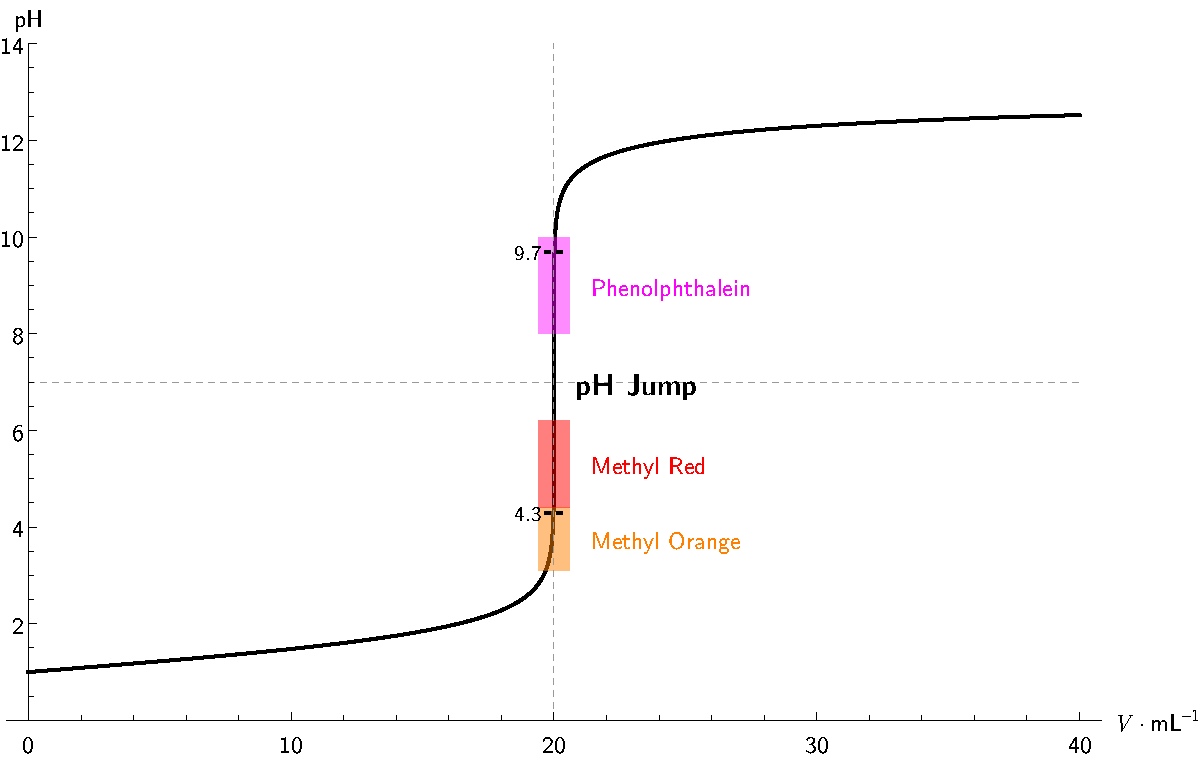
\includegraphics[width=\textwidth]{chapters/titration_indicators_2501.pdf}
            \caption{\SI{0.1}{\mol\per\litre} \cemh{NaOH} 滴定 20.00 mL \SI{0.1}{\mol\per\litre} 盐酸的 pH 变化}
            \label{fig:titration_indicators_2501}
        \end{figure}

        \textcolor{red}{\numrange{4.3}{9.7}，只需要\SI{0.04}{\milli\litre}，即\SI{1}{\text{滴}}溶液（\(\SI{1}{\milli\litre}=\SI{25}{\text{滴}}\)）}

        \textcolor{blue}{指示剂的变色范围要在滴定突跃范围内}

        \textcolor{red}{\(\therefore\)即使过量或不足量，\(\text{误差} \leq \SI{0.02}{\milli\litre}\)（半滴），相对误差 \(\leq \SI{1}{\text{\textperthousand}}\)}

    \subsection{指示剂选择与滴定过程中的颜色变化}\label{subsec:指示剂选择与滴定过程中的颜色变化}

        \begin{enumerate}
            \item 常用酚酞与甲基橙（或甲基红）\footnote{以下分析中甲基橙均可用甲基红替代}；石蕊不宜选用（颜色变化不明显）
            \item 强酸、强碱滴定时，均可选用
            
            \begin{center}
            \begin{tabular}{@{}lcc@{}}
            \toprule
            & 强酸滴强碱 & 强碱滴强酸 \\
            \midrule
            甲基橙 & 黄\(\to\)橙 & 橙\(\to\)红 \\
            酚酞   & 红\(\to\)粉红 & 无\(\to\)粉红 \\
            \bottomrule
            \end{tabular}
            \end{center}
            
            一般：酸滴碱用甲基橙，碱滴酸用酚酞。

            \textcolor{red}{原则：浅色\(\to\)深色}

            \item 强碱滴弱酸
            
            比如：NaOH 溶液滴定醋酸

            \textcolor{red}{原则：反应后盐溶液的酸碱性。选择变色范围接近的指示剂}

            \( \therefore \) 用酚酞

            \item 强酸滴弱碱
            
            用甲基橙或甲基红

        \end{enumerate}

        \begin{figure}[h!]
            \centering
            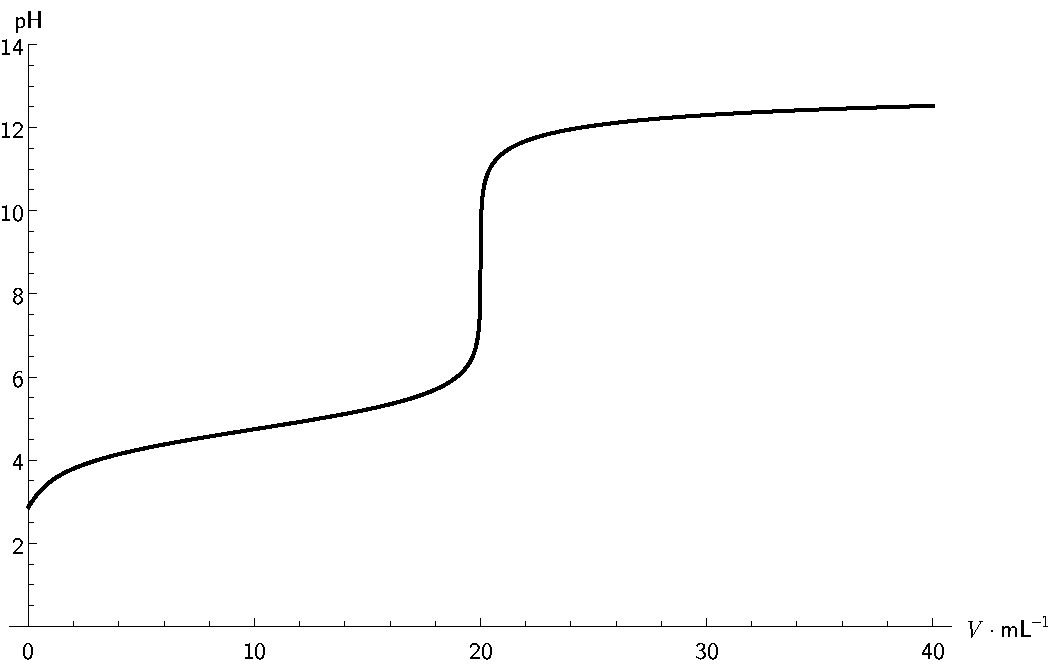
\includegraphics[width=\textwidth]{chapters/titration_acetic_2501.pdf}
            \caption{\SI{0.1}{\mol\per\litre} \cemh{NaOH} 滴定 20.00 mL \SI{0.1}{\mol\per\litre} 醋酸的 pH 变化}
            突跃范围：pH \numrange{7.7}{9.7}
            \label{fig:titration_acetic_2501}
        \end{figure}

    \subsection{误差分析}\label{subsec:误差分析}

        已知：用标准盐酸滴定待测氢氧化钠溶液。下列因素对该实验测定结果是否有影响？如有影响测定结果偏大还是偏小？

        \begin{enumerate}
            \item 滴定时，滴在锥形瓶外一滴盐酸\dotfill\textcolor{blue}{〔偏大〕}
            \item 锥形瓶水洗后直接装入待测 NaOH 溶液\dotfill\textcolor{blue}{〔不变〕}
            \item 锥形瓶水洗后用待测 NaOH 溶液润洗\dotfill\textcolor{blue}{〔偏大〕}
            \item 滴定管水洗后没用待测 NaOH 溶液润洗\dotfill\textcolor{blue}{〔偏小〕}
            \item 滴定管水洗后没有用标准盐酸润洗\dotfill\textcolor{blue}{〔偏大〕}
            \item （碱）开始读数时正确，结束时读数俯视\dotfill\textcolor{blue}{〔偏大〕}
            \item （酸）开始读数时仰视，结束时读数正确\dotfill\textcolor{blue}{〔偏小〕}
            \item （酸）滴定开始读数时未赶走气泡，结束时气泡消失\dotfill\textcolor{blue}{〔偏大〕}
            \item （酸）滴定开始读数时未赶走气泡，结束时仍有气泡\dotfill\textcolor{blue}{〔未知〕}
        \end{enumerate}

    \subsection{典型案例分析}\label{subsec:滴定典型案例分析}

        \begin{xmp}
            [测定小苏打样品的纯度]
            {测定小苏打样品的纯度（杂质为氯化钠）}
            []
            []
            \begin{itemize}
                \item 反应原理：\cemh{NaHCO3 + HCl \xleq{} NaCl + H2O + CO2 ^}
                \item 需要测定的量：样品质量、滴定消耗盐酸体积
                \item 实验步骤：
                \vspace{-0.5\baselineskip}
                \[
                    \overset{\makebox{样品}}{\overset{\makebox{\(\downarrow\)}}{\underset{\makebox{\(m\)\,\si{\gram}}}{\text{称量}}}}
                    \longrightarrow
                    \overset{\makebox{指示剂}}{\overset{\makebox{\(\downarrow\)}}{\underset{}{\text{滴加}}}}
                    \longrightarrow
                    \overset{\makebox[4em][l]{标准盐酸\(c\)\,\si{\mole\per\litre}}}{\overset{\makebox{\(\downarrow\)}}{\underset{\makebox{\(V\)\,\si{\milli\litre}}}{\text{滴定}}}}
                    \phantom{\makebox{\si{\mole\per\litre}}}
                \]

                \item 指示剂应选用：\textcolor{red}{甲基橙或甲基红}
                \item \textcolor{blue}{按\(c=\SI{0.1}{\mole\per\litre}\)、\(V=\SI{10}{\milli\litre}\)}
                
                \textcolor{blue}{计算每次大约称多少克样品：}\textcolor{red}{\SI{0.084}{\gram}}
                
                \textcolor{red}{怎么解决称量太小，称量的相对误差大？}

                \item 实验步骤：\hfil\textcolor{blue}{\( \therefore \) 滴定法测定时，常需要配合使用容量瓶}
                \[
                    \overset{\makebox{样品}}{\overset{\makebox{\(\downarrow\)}}{\underset{\makebox{\(m\)\,\si{\gram}}}{\text{称量}}}}
                    \longrightarrow
                    \overset{\makebox{蒸馏水}}{\overset{\makebox{\(\downarrow\)}}{\underset{\makebox{\(a\)\,\si{\milli\litre}}}{\text{配溶液}}}}
                    \longrightarrow
                    \underset{\makebox{\(b\)\,\si{\milli\litre}}}{\text{量取}}
                    \longrightarrow
                    \overset{\makebox{指示剂}}{\overset{\makebox{\(\downarrow\)}}{\underset{}{\text{滴加}}}}
                    \longrightarrow
                    \overset{\makebox[4em][l]{标准盐酸\(c\)\,\si{\mole\per\litre}}}{\overset{\makebox{\(\downarrow\)}}{\underset{\makebox{\(V\)\,\si{\milli\litre}}}{\text{滴定}}}}
                    \phantom{\makebox{\si{\mole\per\litre}}}
                \]

                \item 计算式：
                \vspace{-1.5\baselineskip}

                \[
                    \cemh{NaHCO3}\si{\percent}=\frac{\frac{c\cdot V}{1000} \times \frac{a}{b} \times 84}{m} \times \SI{100}{\percent}
                \]
            \end{itemize}
        \end{xmp}
    
        \begin{xmp}
            [返滴定法]
            {测定鸡蛋壳中的 \cemh{CaCO3} 含量（返滴定法）}
            []
            []
            \textcolor{red}{无法直接滴定，如何用滴定法测定？能否转换成酸碱滴定？}
            \begin{itemize}
                \item 反应原理：\cemh{CaCO3 + 2HCl \xleq{} CaCl2 + H2O + CO2 ^}
                
                \phantom{反应原理：}\cemh{HCl + NaOH \xleq{} NaCl + H2O}
                \item 实验步骤：
                \vspace{-0.5\baselineskip}
                \[
                    \text{鸡蛋壳}
                    \longrightarrow
                    \text{粉碎}
                    \longrightarrow
                    \text{称量}
                    \longrightarrow
                    \overset{\makebox{足量盐酸}}{\overset{\makebox{\(\downarrow\)}}{\underset{}{\text{酸溶}}}}
                    \longrightarrow
                    \overset{\makebox{蒸馏水}}{\overset{\makebox{\(\downarrow\)}}{\underset{\makebox{\(a\)\,\si{\milli\litre}}}{\text{配溶液}}}}
                    \longrightarrow
                \]
                \[
                    \longrightarrow
                    \underset{\makebox{\(b\)\,\si{\milli\litre}}}{\text{量取}}
                    \longrightarrow
                    \overset{\makebox{指示剂}}{\overset{\makebox{\(\downarrow\)}}{\underset{}{\text{滴加}}}}
                    \longrightarrow
                    \overset{\makebox{标准 \cemh{NaOH} 溶液}}{\overset{\makebox{\(\downarrow\)}}{\underset{}{\text{滴定}}}}
                \]

                \item 计算需要的物理量：鸡蛋壳的质量、盐酸的浓度和体积、\cemh{NaOH} 溶液的浓度和体积
            \end{itemize}
        \end{xmp}

    \subsection[氧化还原滴定]{氧化还原滴定——利用氧化还原反应的滴定测定法}\label{subsec:拓展：氧化还原滴定}

        \subsubsection{高锰酸钾法}\label{subsubsec:高锰酸钾法氧化还原滴定}

            \textcolor{red}{需酸化，通常用 \cemh{H2SO4}，不使用 \cemh{HCl} 或 \cemh{HNO3}}

            \vspace{-0.5\baselineskip}
            \[\cemh{MnO4- + 5 e- + 8H+ \xleq{} Mn^2+ + 4H2O}\]

            \textcolor{blue}{优点：氧化能力强、可测定物质多，一般不需要另加指示剂}

            \begin{enumerate}
                \item 直接滴定
                
                测定还原性物质，如：\cemh{Fe^2+}、\cemh{H2O2}、\cemh{H2C2O4}、\cemh{Sn^2+} 等

                滴定终点判断：当滴入最后半滴后，溶液显浅紫红色，\uline{并保持半分钟不复原}

                \item 返滴定
                
                测定氧化性物质，如：\cemh{MnO2}、\cemh{Pb2O4}、\cemh{K2Cr2O7}、\cemh{KClO3} 等

                \begin{xmp}
                    [软锰矿中 MnO2 的含量测定]
                    {软锰矿中 \cemh{MnO2} 的含量测定}
                    []
                    []
                    在 \cemh{H2SO4} 存在下，加入一定量且过量的 \cemh{Na2C2O4}，加热充分反应后，用标准 \cemh{KMnO4} 溶液滴定过量的 \cemh{C2O4^2-}。
                \end{xmp}

                \item 间接滴定
                
                \begin{xmp}
                    [Ca2+含量测定]
                    {\cemh{Ca^2+} 含量测定}
                    []
                    []
                    首先用 \cemh{C2O4^2-} 将 \cemh{Ca^2+} 沉淀为 \cemh{CaC2O4}，过滤，再用稀 \cemh{H2SO4} 将 \cemh{CaC2O4} 沉淀溶解，然后用标准 \cemh{KMnO4} 溶液滴定 \cemh{H2C2O4}，从而间接求得 \cemh{Ca^2+} 含量。
                \end{xmp}

            \end{enumerate}
            
        \subsubsection{碘量法}\label{subsubsec:碘量法氧化还原滴定}
        
            \textcolor{blue}{用淀粉溶液作指示剂}

            \begin{enumerate}
                \item 直接碘量法\textcolor{red}{（碘标准溶液）}
                
                测定较强的还原剂，如：\cemh{S^2-}、\cemh{SO3^2-}、\cemh{Sn^2+}、\cemh{V_C} 等

                例如 \cemh{V_C} 与 \cemh{I2} 反应： \cemh{C6H8O6 + I2 -> C6H6O6 + 2HI}

                滴定终点判断：当滴入最后半滴后，溶液显蓝色，\uline{并保持半分钟不复原}

                \item 间接碘量法\textcolor{red}{（\cemh{Na2S2O3} 标准溶液）}
                
                测定氧化性物质，如 \cemh{H2O2}、\cemh{Cu^2+}、\cemh{KIO3}、\cemh{NaClO} 等

                先与过量的 \cemh{KI} 反应生成 \cemh{I2}，用 \cemh{Na2S2O3} 标准溶液滴定生成的 \cemh{I2}，从而计算得到氧化性物质的量。\cemh{2S2O3^2- + I2 \xleq{} S4O6^2- + 2I-}

                滴定终点判断：当滴入最后半滴后，溶液蓝色褪去，\uline{并保持半分钟不复原}

                注意事项：
                \begin{enumerate}
                    \item 加入过量的 \cemh{KI}，形成 \cemh{I3-}（\cemh{I- + I2 \xleq{} I3-}），降低 \cemh{I2} 的挥发性
                    \item 由于 \cemh{I-} 易被 \cemh{O2} 氧化，滴定时不宜剧烈摇动锥形瓶
                \end{enumerate}

            \end{enumerate}


\section{\S 3.4 沉淀溶解平衡}\label{sect:沉淀溶解平衡}

    \begin{itemize}
        \item \cemh{AgCl <=> Ag+ + Cl^-} 是哪种平衡？
        \item \cemh{NaCl_{(s)} <=> Na^+_{(aq)} + Cl^-_{(aq)}} 又是哪种平衡？
        \item \cemh{3Mg(OH)2 + 2FeCl3 \xleq{} 3MgCl2 + 2Fe(OH)3} 能发生吗？
        \item \cemh{Fe^{3+}} 在 \(\text{pH}=5\) 的溶液中能存在吗？
    \end{itemize}

    \textcolor{red}{我们如何判断某种金属正离子在 pH 一定的溶液中能否存在？}

    \subsection*{溶解平衡\textcolor{red}{——也是动态平衡}}\label{subsec:溶解平衡}

        \vspace{-\baselineskip}
            \[ \cemh{\text{固体溶质} <=>[\text{结晶}][\text{溶解}] \text{溶液中的溶质}}
            \quad \cemh{\text{气体分子} <=>[\text{析出}][\text{溶解}] \text{溶液中的微粒}} \]

        \begin{itemize}
            \item \(V_\text{溶解} > V_\text{结晶}\)\quad 溶质不断溶解减少（不饱和溶液）
            \item \(V_\text{溶解} = V_\text{结晶}\)\quad 溶质量不变，达到溶解平衡（饱和溶液）
            \item \(V_\text{溶解} < V_\text{结晶}\)\quad 溶质结晶析出，直至重新达到溶解平衡
        \end{itemize}

        溶解平衡的建立\textcolor{red}{——必须饱和溶液}

        \textcolor{blue}{\(\therefore\)难溶电解质的溶解平衡容易建立}

        难溶物：溶解度 \(< \SI{0.01}{g}/100\text{g 水}\)

        \textcolor{red}{难溶电解质，如何比较它们的溶解度大小？}

        \[ \cemh{AgCl_{(s)} <=>[\text{溶解}][\text{沉淀}] Ag^+_{(aq)} + Cl^-_{(aq)}} \]

        当\(v_\text{溶解} = v_\text{沉淀}\)时，实现平衡状态——沉淀溶解平衡

    \subsection[溶度积常数]{溶度积常数（简称：溶度积；符号：\(K_{\text{sp}}\)）}\label{subsec:溶度积常数}

        对于 \cemh{AgCl_{(s)}}，\( K_\text{sp} = \cemh{[Ag+]} \cdot \cemh{[Cl^-]} \quad K_\text{sp}(\cemh{AgCl}) = \cemh{[Ag+]} \cdot \cemh{[Cl^-]} \) 

        对于难溶电解质 \cemh{A_mB_n}，\cemh{A_mB_n_{(s)} <=> m A^{n+}_{(aq)} + n B^{m-}_{(aq)}}
        \[ K_\text{sp} = \cemh{[A^{n+}]}^m \cdot \cemh{[B^{m-}]}^n \]

        \subsubsection{溶度积与溶解度的关系}\label{subsubsec:溶度积与溶解度的关系}
            
            对于 \cemh{AB} 型难溶电解质，\( s = \sqrt{K_\text{sp}} \)\footnote{\(s_0(\si{\gram/100\gram\text{水}}) = \dfrac{s(\si{\mole\per\litre}) \cdot M}{10}\)}

            对于 \cemh{A2B} 型或 \cemh{AB2} 型难溶电解质，\( s = \sqrt[3]{\frac{K_\text{sp}}{4}} \)

            \textcolor{blue}{对于同类型难溶电解质，\(K_{\text{sp}}\)越小，在水中的溶解度也越小}
            
            \textcolor{blue}{不同类型，不能直接用\(K_{\text{sp}}\)比较，若相差很大，依然可以快速判断}

        \subsubsection{\texorpdfstring{\(K_{\text{sp}}\)}{Kₛₚ}的意义和影响因素}\label{subsubsec:Ksp意义和影响因素}
            
            \(K_{\text{sp}}\)的大小也反映了难溶电解质溶解趋势的大小，也反映了其生成沉淀的难易程度\textcolor{blue}{（越小越易生成）}
            
            \begin{xmp}
                [Ksp 意义]
                {}
                []
                []
                在含有 \cemh{Cl^-}、\cemh{Br-}、\cemh{I-} 的混合溶液中，滴加 \cemh{AgNO3} 溶液，最先生成 \cemh{AgI} 沉淀，最后生成 \cemh{AgCl} 沉淀。
            \end{xmp}

            \(K_{\text{sp}}\)的影响因素\(\left\{\begin{matrix} \makebox[1em][l]{难溶电解质本身的溶解度} \\
                \makebox[1em][l]{温度\textcolor{blue}{（大多数随温度升高而增大）}} \end{matrix}\right.\)

            \textcolor{red}{不受离子浓度影响}

        \subsubsection{溶度积规则}\label{subsubsec:溶度积规则}

            对于难溶电解质 \cemh{A_mB_n}，\cemh{A_mB_n_{(s)} <=> m A^{n+}_{(aq)} + n B^{m-}_{(aq)}}

            离子积\(Q\)，\(Q = c^m(\cemh{A^{n+}}) \cdot c^n(\cemh{B^{m-}})\)
            \begin{itemize}
                \item $Q < K_{sp}$时，无沉淀析出
                \item $Q = K_{sp}$时，沉淀溶解平衡状态
                \item $Q > K_{sp}$时，有沉淀析出，直至平衡状态
            \end{itemize}

        \begin{xmp}
            [沉淀生成判断]
            {}
            []
            []
            向 \SI{5}{\milli\litre} \SI{0.002}{\mole\per\litre} 的 \cemh{BaCl2} 溶液中加入 \SI{5}{\milli\litre} \SI{0.002}{\mole\per\litre} 的 \cemh{Na2SO4} 溶液，\Circled{1}计算判断是否有沉淀生成；\Circled{2}\cemh{Ba^{2+}}是否沉淀完全；\Circled{3}\cemh{Na2SO4} 溶液浓度改为\SI{0.0022}{\mole\per\litre}。\footnote{\textcolor{blue}{注：当溶液中离子浓度小于\textcolor{red}{\SI{E-5}{\mole\per\litre}} 时，即认为沉淀完全。}}
            
            （已知\(K_\text{sp}(\cemh{BaSO4}) = \num{1.08E-10}\)）
        \end{xmp}

        \begin{xmp}
            [同离子效应计算]
            {}
            []
            []
            计算 \cemh{BaSO4} 固体在下列条件下的溶解度（\si{\mole\per\litre}）\Circled{1}纯水中；\Circled{2}\SI{0.10}{\mole\per\litre} \cemh{Na2SO4} 溶液中；\Circled{3}\SI{0.001}{\mole\per\litre}的 \cemh{BaCl2} 溶液中。

            （已知\(K_\text{sp}(\cemh{BaSO4}) = \num{1.08E-10}\)）
            
            \Circled{1} \SI{1.04E-5}{\mole\per\litre}
            
            \Circled{2} \SI{1.08E-9}{\mole\per\litre}
            
            \Circled{3} \SI{1.08E-8}{\mole\per\litre}
            
        \end{xmp}

        \textcolor{blue}{同离子效应}：含有相同离子的易溶强电解质时，沉淀溶液平衡逆向移动，难溶电解质的溶解度减小。

        \textcolor{red}{\(\therefore\)沉淀剂往々会加过量}

        \subsubsection{难溶氢氧化物的开始沉淀 pH 和完全沉淀 pH}\label{subsubsec:难溶氢氧化物的开始沉淀pH和完全沉淀pH}

            金属离子的浓度为\SI{0.1}{\mole\per\litre}

            \begin{tabular}{|c|c|c|c|c|}
                \hline
                离子 & 氢氧化物 & 溶度积 \(K_{\text{sp}}\) & 开始沉淀 pH & 完全沉淀 pH \\
                \hline
                \cemh{Fe^{3+}} & \cemh{Fe(OH)3} & \num{2.79E-39} & 1.82& 2.82 \\
                \hline
                \cemh{Fe^{2+}} & \cemh{Fe(OH)2} & \num{4.87E-17} & 6.84 & 8.34 \\
                \hline
                \cemh{Cu^{2+}} & \cemh{Cu(OH)2} & \num{2.2E-20} & 5.17 & 6.67 \\
                \hline
                \cemh{Mg^{2+}} & \cemh{Mg(OH)2} & \num{8.45E-12} & 9.46 & 10.96 \\
                \hline
                \cemh{Al^{3+}} & \cemh{Al(OH)3} & \num{1.1E-33} & 3.68 & 4.68 \\
                \hline
            \end{tabular}

            \cemh{Fe(OH)3_{(s)} <=> Fe^{3+}_{(aq)} + 3OH^-_{(aq)}}

            \( \displaystyle K_\text{sp}(\cemh{Fe(OH)3}) = \cemh{[Fe^{3+}]} \cdot \cemh{[OH^-]}^3 \quad \cemh{[OH^-]} = \sqrt[3]{\frac{K_{\text{sp}}}{\cemh{[Fe^{3+}]}}} \quad \cemh{[H^+]} = \frac{K_\text{W}}{\cemh{[OH^-]}} \)

            \begin{xmp}
                [分离除杂应用]
                {}
                []
                []
                在酸化的 \cemh{CuSO4} 溶液中混有 \cemh{Fe^{3+}}，可加入\uline{\makebox[3em]{\cemh{CuO}}}来提高溶液的 pH，可以使 \cemh{Fe^{3+}}转变为 \cemh{Fe(OH)3} 而除去。该物质是否可以加过量？

                若还有 \cemh{Fe^{2+}}，可以先加入\uline{\makebox[3em]{\cemh{H2O2}}}，后再加入以上物质。

                \begin{enumerate}
                    \item \textcolor{red}{能与 \cemh{H+} 反应}
                    \item \textcolor{red}{不引入其他杂质离子\quad \(\therefore\)是含铜化合物}
                    \item \textcolor{red}{本身是难溶物，过量也可过滤除去}
                \end{enumerate}
                \begin{enumerate}
                    \item \textcolor{blue}{能够氧化 \cemh{Fe^{2+}}}
                    \item \textcolor{blue}{不引入杂质}
                \end{enumerate}
            \end{xmp}

    \subsection{沉淀溶解平衡的移动}\label{subsec:沉淀溶解平衡的移动}

        \subsubsection{常见金属离子沉淀物的颜色}\label{subsubsec:常见金属离子沉淀物的颜色}

            \begin{center}
            \small
            \begin{tabular}{|c|c|c|c|}
                \hline
                银盐或硫化物 & 颜色 & 氢氧化物 & 颜色 \\
                \hline
                氯化银 & 白色 & 氢氧化镁 & 白色 \\
                \hline
                溴化银 & 淡黄色 & 氢氧化铝 & 白色 \\
                \hline
                碘化银 & 黄色 & 氢氧化铜 & 黄色 \\
                \hline
                硫化银 & 黑色 & 氢氧化铁 & 红褐色 \\
                \hline
                硫化锌 & 白色 & 氢氧化亚铁 & 白色 \\
                \hline
            \end{tabular}
            \end{center}

        \subsubsection{沉淀的转化}\label{subsubsec:沉淀的转化}

            \makebox[20em][l]{\cemh{AgCl_{(s)} <=> Ag^+_{(aq)} + Cl^-_{(aq)}}} \(K_1 = K_\text{sp}(\cemh{AgCl})\)

            \makebox[20em][l]{\cemh{Ag^+_{(aq)} + I^-_{(aq)} <=> AgI_{(s)}}} \(K_2 = \frac{1}{K_\text{sp}(\cemh{AgI})}\)

            \cemh{AgCl_{(s)} + I^-_{(aq)} \xleq{} AgI_{(s)} + Cl^-_{(aq)}}

            \textcolor{red}{该过程的进行程度有多大？}

            \textcolor{blue}{方法一}：
            \[
                K = \frac{\cemh{[Cl^-]}}{\cemh{[I^-]}} = \frac{\cemh{[Cl^-]}\cdot\cemh{[Ag+]}}{\cemh{[I^-]}\cdot\cemh{[Ag+]}} = \frac{K_\text{sp}(\cemh{AgCl})}{K_\text{sp}(\cemh{AgI})} = \frac{\num{1.77E-10}}{\num{8.51E-17}} = \num{2.08E6}
            .\]

            \textcolor{blue}{方法二}：
            \[
                K = K_1 \times K_2 = \frac{K_\text{sp}(\cemh{AgCl})}{K_\text{sp}(\cemh{AgI})}
            .\]
            \textcolor{red}{\(\therefore\)该转化进行程度很大}


            \cemh{2AgI_{(s)} + S^{2-}_{(aq)} \xleq{} Ag2S_{(s)} + 2I^-_{(aq)}}

            \textcolor{red}{该过程的进行程度有多大？}

            \textcolor{blue}{方法一}：
            \[
                K = \frac{\cemh{[I^-]}^2}{\cemh{[S^{2-}]}} = \frac{\cemh{[I^-]}^2\cdot\cemh{[Ag+]}^2}{\cemh{[S^{2-}]}\cdot\cemh{[Ag+]}^2} = \frac{(K_\text{sp}(\cemh{AgI}))^2}{K_\text{sp}(\cemh{Ag2S})} = \frac{\left(\num{8.51E-17}\right)^2}{\num{6.69E-50}} = \num{1.08E17}
            .\]
            \textcolor{red}{\(\therefore\)该转化进行程度极大}

            \textcolor{blue}{方法二}：

            \makebox[20em][l]{\cemh{2AgI_{(s)} <=> 2Ag^+_{(aq)} + 2I^-_{(aq)}}} \(K_1 = (K_\text{sp}(\cemh{AgI})^2)\)

            \makebox[20em][l]{\cemh{2Ag^+_{(aq)} + S^{2-}_{(aq)} <=> Ag2S_{(s)}}} \(K_2 = \frac{1}{K_\text{sp}(\cemh{Ag2S})}\)

            \[
                K = K_1 \times K_2 = \frac{(K_\text{sp}(\cemh{AgI}))^2}{K_\text{sp}(\cemh{Ag2S})}
            .\]

            \textcolor{blue}{一般来说，同种离子的难溶物，溶解度小的易转化成溶解度更小的；\(K_\text{sp}\)小相差越大，转化越完全。}


            \cemh{3Mg(OH)2 + 2FeCl3 \xleq{} 3MgCl2 + 2Fe(OH)3}

            \textcolor{red}{这个反应能发生吗？进行程度大吗？}

            \[
                K = \frac{(K_\text{sp}(\cemh{Mg(OH)2}))^3}{(K_\text{sp}(\cemh{Fe(OH)3}))^2} = \frac{\left(\num{8.45E-12}\right)^3}{\left(\num{2.79E-39}\right)^2} = \num{7.75E43}
            .\]

            \textcolor{red}{【归纳】}

            沉淀转化反应的\(K = \frac{\left(\text{前一个沉淀的}K_\text{sp}\right)^\text{幂次方}}{\left(\text{后一个沉淀的}K_\text{sp}\right)^\text{幂次方}}\)
            

            \begin{xmp}
                [硫酸亚铁混有亚铜离子]
                {应用实例}
                []
                []
                硫酸亚铁溶液中混有 \cemh{Cu2+}，如何除去？

                可以通过加入 \cemh{FeS} 充分反应后过滤除去。

                \[
                    \cemh{FeS_{(s)} + Cu^{2+}_{(aq)} \xleq{} CuS_{(s)} + Fe^{2+}_{(aq)}}
                ,\]

                \[
                    K = \frac{K_\text{sp}(\cemh{FeS})}{K_\text{sp}(\cemh{CuS})} = \frac{\num{1.59E19}}{\num{1.27E36}} = \num{1.25E17}
                .\]
            \end{xmp}

            \textcolor{blue}{沉淀转化当\(K_\text{sp}\)接近时，则取决于离子浓度}

            \begin{xmp}
                [Ksp 接近时的判据]
                {}
                []
                []
                \cemh{BaSO4_{(s)} + CO3^{2-}_{(aq)} <=> BaCO3_{(s)} + SO4^{2-}_{(aq)}}

                \[
                    K = \frac{\cemh{[SO4^{2-}]}}{\cemh{[CO3^{2-}]}} = \frac{K_\text{sp}(\cemh{BaSO4})}{K_\text{sp}(\cemh{BaCO3})} = \frac{\num{1.08E-10}}{\num{8.1E-9}} = \frac{1}{75}
                .\]

                \(\therefore\)当\(c(\cemh{CO_3^{2-}}) > 75c(\cemh{SO_4^{2-}})\)时，\(Q = \frac{c{\cemh{SO_4^{2-}}}}{c{\cemh{CO_3^{2-}}}} < \frac{1}{75} = K\)，反应正向进行。
            \end{xmp}

        \subsubsection{沉淀的溶解}\label{subsubsec:沉淀的溶解}

            \noindent\textbf{（1）氢氧化物溶于酸（生成水）}
            
            \cemh{Mg(OH)2_{(s)} <=> Mg^{2+}_{(aq)} + 2OH^-_{(aq)}}

            \cemh{2H^+_{(aq)} + 2OH^-_{(aq)} \xleq{} 2H2O_{(l)}}
            
            \cemh{Mg(OH)2_{(s)} + 2H^+_{(aq)} \xleq{} Mg^{2+}_{(aq)} + 2H2O_{(l)}}
            
            \textcolor{red}{计算常温下该反应的\(K\)}
            \[
                K = \frac{K_\text{sp}(\cemh{Mg(OH)2})}{K_\text{W}^2} = \frac{8.45E-12}{\left(1.0E-14\right)^2} = \num{8.45E16}
            .\]

            \noindent\textbf{（2）碳酸盐溶于酸（生成气体）}

            \cemh{CaCO3_{(s)} + 2H^+_{(aq)} <=> Ca^{2+}_{(aq)} + H2CO3_{(aq)}}

            \textcolor{red}{计算常温下该反应的\(K\)}
            \[
                K = \frac{K_\text{sp}(\cemh{CaCO3})}{K_\text{a1}(\cemh{H2CO3})\cdot K_\text{a2}(\cemh{H2CO3})} = \frac{4.96E-9}{\num{4.2E-7}\cdot\num{4.8E-11}} = 2.46E8
            .\]
            \cemh{H2CO3_{(aq)} \xleq{} H2O_{(l)} + CO2_{(g)}}
            
            再考虑 \cemh{CO2_{(g)}}的逸出，实际\(K\)还要大。

            \noindent\textbf{（3）氢氧化镁溶于浓氯化铵（生成弱电解质）}

            \cemh{Mg(OH)2_{(s)} + 2NH4^+_{(aq)} <=> Mg^{2+}_{(aq)} + 2NH3 . H2O_{(aq)}}

            \[
                K = \frac{K_\text{sp}(\cemh{Mg(OH)2})}{(K_\text{b}(\cemh{NH3 . H2O}))^2} = \frac{\num{8.45E-12}}{(\num{1.8E-5})^2} = 0.026
            .\]

            \textcolor{red}{\(\therefore\)需要浓的氯化铵溶液才能溶解氢氧化镁}

            \noindent\textbf{（4）氯化银溶于氨水（生成配合物）}

            \cemh{AgCl_{(s)} + 2NH3_{(aq)} <=> [Ag(NH3)2]^+_{(aq)} + Cl^-_{(aq)}}

            \makebox[20em][l]{\cemh{AgCl_{(s)} <=> Ag^+_{(aq)} + Cl^-_{(aq)}}} \(K_\text{sp}(\cemh{AgCl})\)

            \makebox[20em][l]{\cemh{Ag^+_{(aq)} + 2NH3_{(aq)} <=> [Ag(NH3)2]^+_{(aq)}}} \(K_\text{稳}(\cemh{[Ag(NH3)2]+})\)

            \noindent\textbf{（5）难溶金属硫化物是否都溶于强酸}

            \cemh{FeS_{(s)} + 2H^+_{(aq)} <=> H2S_{(aq)} + Fe^{2+}_{(aq)}}

            \[
                K = \frac{K_\text{sp}(\cemh{FeS})}{K_\text{a1}(\cemh{H2S})\cdot K_\text{a2}(\cemh{H2S})} = \frac{\num{1.59E-19}}{\num{5.7E-8}\cdot\num{1.2E-15}} = \num{2.32E3}
            .\]

            \cemh{CuS_{(s)} + 2H^+_{(aq)} <=> H2S_{(aq)} + Cu^{2+}_{(aq)}}

            \[
                K = \frac{K_\text{sp}(\cemh{CuS})}{K_\text{a1}(\cemh{H2S})\cdot K_\text{a2}(\cemh{H2S})} = \frac{\num{1.27E-36}}{\num{5.7E-8}\cdot\num{1.2E-15}} = \num{1.86E-14}
            .\]

            \textcolor{red}{\(\therefore\)\cemh{FeS} 溶于强酸，\cemh{CuS} 不溶}

    \subsection*{如何衡量判断竞争反应}\label{subsec:竞争反应判断}
    \addcontentsline{toc}{subsection}{如何衡量判断竞争反应}
        \textcolor{red}{——利用常数}


\input{chapters/2501/2501-07}

\section{\S 2.1 Explain the Molecular Structure by VSEPR and Hybrid Orbital Theory}\label{sect:VSEPR和杂化轨道理论}

    \subsection{价层电子对互斥理论（VSEPR）}\label{subsec:VSEPR}

        \begin{itemize}
            \item \makebox[10em][l]{\textbf{\uline{V}alence}}价
            \item \makebox[10em][l]{\textbf{\uline{S}hell}}层
            \item \makebox[10em][l]{\textbf{\uline{E}lectron}}电子
            \item \makebox[10em][l]{\textbf{\uline{P}air}}对
            \item \makebox[10em][l]{\textbf{\uline{R}epulsion}}排斥
        \end{itemize}

        能够解释、判断简单共价分子和（含共价键的）离子的几何构型。

        主要适用于 \(AB_n\) 型分子或离子

        \begin{itemize}
            \item A——中心原子
            \item B——配位原子
            \item n——配位原子个数
        \end{itemize}

        \subsubsection{理论基本观点}\label{subsubsec:VSEPR基本观点}

            中心原子的价层电子对由于相互间的排斥作用，尽可能彼此远离，使电子对之间的静电斥力最小，体系能量最低，分子最稳定。

            价层电子对包括：成键 \(\upsigma\) 电子对和孤电子对

        \subsubsection{价层电子对的排列方式}\label{subsubsec:价层电子对排列方式}

            \begin{center}
            \begin{tabular}{|c|c|c|c|c|c|c|}
                \hline
                \noindent\textbf{价层电子对数} & \textbf{2对} & \textbf{3对} & \textbf{4对} & \textbf{5对} & \textbf{6对} \\
                \hline
                \makecell{VSEPR \\ 理论模型} & 直线形 & 平面正三角形 & 正四面体形 & & \\
                \hline
                \makecell{中心原子 \\ 杂化方式} & sp & sp$^2$ & sp$^3$ & & \\
                \hline
            \end{tabular}
            \end{center}

        \subsubsection{确定价层电子对数}\label{subsubsec:确定价层电子对数}

            价层电子对数 =
            \[\underset{\text{成键}\upsigma\text{电子对数}}{n} + (\underset{\text{孤电子对数}}{\text{A的价电子数}} - \overset{\makebox[0pt]{\footnotesize 代数值}}{\text{离子电荷}} - n \times \text{B的单电子数})\div 2\]

            或：\quad   \(\begin{cases} - \text{ 正离子电荷数} \\ + \text{ 负离子电荷数} \end{cases}\)

            \begin{xmp}{价层电子对数计算}
                计算下列分子或离子的价层电子对数。
                
                \cemh{CO2}：\(2 + 0 = 2\)对\qquad \cemh{PCl3}：\(3 + 1 = 4\)对\qquad \cemh{SO2}：\(2 + 1 = 3\)对
                \qquad \cemh{NH4+}：\(4 + 0 = 4\)对\qquad \cemh{CO3^{2-}}：\(3 + 0 = 3\)对
            \end{xmp}

        \subsubsection{实例分析}\label{subsubsec:VSEPR实例分析}

            \begin{center}
            \small
            \begin{tabular}{|c|c|c|c|c|c|}
                \hline
                \noindent\textbf{\makecell{价层电子\\对数}} & \textbf{\makecell{VSEPR\\模型}} & \textbf{\makecell{成键\(\upsigma\)\\电子对数}} & \textbf{\makecell{孤电子\\对数}} & \textbf{实例} & \textbf{分子几何构型} \\
                \hline
                \multirow{1}{*}{2} & 直线形 & 2 & 0 & \makecell{\cemh{BeCl2}, \cemh{CO2}} & 直线形 \\
                \hline
                \multirow{2}{*}{3} & 正三角形 & 3 & 0 & \makecell{\cemh{BF3}, \cemh{CO3^{2-}}} & 正三角形 \\
                \cline{3-6}
                & 三角形 & 2 & 1 & \cemh{SO2} & \makecell{角形 \\\footnotesize（折线形、V字形）} \\
                \hline
                \multirow{3}{*}{4} & 正四面体形 & 4 & 0 & \makecell{\cemh{CCl4}, \cemh{CH4},\\\cemh{NH4+}} & 正四面体形 \\
                \cline{3-6}
                & 四面体形 & 3 & 1 & \makecell{\cemh{NH3}, \cemh{PCl3},\\\cemh{PH3}} & 三角锥形 \\
                \cline{3-6}
                & 四面体形 & 2 & 2 & \makecell{\cemh{H2O}, \cemh{H2S}} & \makecell{角形 \\\footnotesize（折线形、V字形）} \\
                \hline
            \end{tabular}
            \end{center}

            \noindent\textbf{总结}
            \begin{itemize}
                \item \textcolor{blue}{先计算出价层电子对总数，确定VSEPR模型；}
                \item \textcolor{blue}{若孤电子对数 = 0，则分子的空间构型即为VSEPR模型；}
                \item \textcolor{blue}{若孤电子对数 \(\neq\) 0，则从VSEPR模型扣除相应的顶点数，判断剩余原子组成的空间构型。}
            \end{itemize}

        \subsubsection{影响键角的因素}\label{subsubsec:影响键角的因素}

        \vspace{-\baselineskip}
            \begin{align*}
                \cemh{CH4} \text{键角：} & \ang{109;28} \\
                \cemh{NH3} \text{键角：} & \ang{107;18} \\
                \cemh{H2O} \text{键角：} & \ang{104.5}
            \end{align*}

            都是4对价层电子对，相同的VSEPR模型，为什么键角不同？

            \textcolor{red}{斥力大小}：lp-lp \(>\) lp-bp \(>\) bp-bp\quad \(\longleftarrow\)\textcolor{red}{为什么？}

            （lp：孤电子对 lonely pair；bp：成键电子对 bonding pair）

            \textcolor{blue}{\(\therefore\) 键角：\cemh{H2O} \(<\) \cemh{NH3} \(<\) \cemh{CH4}}

            \begin{xmp}{分子构型分析}
                分析下列分子的空间构型
                
                \cemh{HCN} \(2 + 0 = 2\)对，\textcolor{blue}{直线形}
            
                \cemh{HClO} \cemh{HOCl} \(2 + 2 = 4\)对，\textcolor{blue}{角形}
                
                \cemh{COCl2} \(3 + 0 = 3\)对，\textcolor{blue}{平面三角形}

                \textcolor{red}{斥力大小}：三键 \(>\) 双键 \(>\) 单键\quad \(\longleftarrow\)\textcolor{red}{为什么？}
            \end{xmp}

            知道分子的空间结构，能否帮助我们分析分子的成键方式？

            \begin{xmp}{空间构型练习}
                分析下列分子或离子的空间构型
                
                \cemh{SO3} \(3 + 0 = 3\)对，\textcolor{blue}{平面正三角形}
                
                \cemh{SO4^{2-}} \(4 + 0 = 4\)对，\textcolor{blue}{正四面体形}
                
                \cemh{NF3} \(3 + 1 = 4\)对，\textcolor{blue}{三角锥形}
            \end{xmp}

            \noindent\textbf{比较下列分子的键角大小}

            \makebox[0.5\textwidth][l]{\Circled{1} 对于\cemh{H2O}和\cemh{H2S}}\Circled{2} 对于\cemh{NH3}和\cemh{NF3}

            % transposed table inserted below
            \begin{center}
            \small
            \begin{tabular}{|c|c|c|c|c|}
                \hline
                \noindent\textbf{分子} & \cemh{H2O} & \cemh{H2S} & \cemh{NH3} & \cemh{NF3}\\
                \hline
                \noindent\textbf{键角} & \ang{104.5} & \ang{92.2} & \ang{107.3} & \ang{102}\\
                \hline
            \end{tabular}
            \end{center}

            一般来说：中心原子电负性越大，键角越大

            \phantom{一般来说：}配位原子电负性越大，键角越小

    \subsection{杂化轨道理论分析分子或复杂离子的结构}\label{subsec:杂化轨道理论}

        \noindent\textbf{归纳：}
        \begin{enumerate}
            \item 先由价层电子对数判断杂化方式。
            \item 几个配位原子形成几根 \(\upsigma\) 键。
            \item 结合VSEPR模型和配位原子数分析空间结构。
            \item sp$^2$杂化，分析垂直于成键原子平面的p轨道如何形成\(\uppi\)键。
            \item sp杂化，分析垂直于键轴的p轨道如何形成\(\uppi\)键。
            \item 若有多个原子的p轨道均垂直，则形成离域\(\uppi\)键。
        \end{enumerate}

        \textcolor{red}{一般不分析末端原子的杂化方式（大多数时候其实也杂化）。}

        \subsubsection{实例：直线形分子}\label{subsubsec:直线形分子}

            \noindent\begin{minipage}[t]{0.48\textwidth}
                \noindent\textbf{\cemh{BeCl2}}
                
                VSEPR模型：直线形
                
                Be原子 sp 杂化
                
                \(\therefore\) \cemh{BeCl2}直线形
                
                \vspace{\baselineskip}
            
                \noindent\textbf{\cemh{HCN}}
                
                VSEPR模型：直线形
                
                C原子 sp 杂化
                
                \cemh{H-C#N}
                
                \(\therefore\) \cemh{HCN}直线形
            \end{minipage}
            \hfill
            \begin{minipage}[t]{0.48\textwidth}
                \noindent\textbf{\cemh{CO2}}
                
                VSEPR模型：直线形
                
                C原子 sp 杂化
                
                \cemh{CO2}分子中含有2根\(\upsigma\)键、2根\(\uppi\)键
                
                \(\therefore\) \cemh{CO2}直线形
            \end{minipage}

        \subsubsection{实例：平面三角形分子}\label{subsubsec:平面三角形分子}

            \noindent\begin{minipage}[t]{0.48\textwidth}
                \noindent\textbf{\cemh{BF3}}
                
                VSEPR模型：平面正三角形
                
                B原子 sp$^2$ 杂化
                
                \(\therefore\) \cemh{BF3}平面正三角形
            \end{minipage}
            \hfill
            \begin{minipage}[t]{0.48\textwidth}
                \noindent\textbf{\cemh{CO3^{2-}}}
                
                VSEPR模型：平面正三角形
                
                C原子 sp$^2$ 杂化
            \end{minipage}

        \subsubsection{实例：四面体形分子}\label{subsubsec:四面体形分子}

            \noindent\begin{minipage}[t]{0.48\textwidth}
                \noindent\textbf{\cemh{CH4}、\cemh{CF4}}
                
                VSEPR模型：正四面体形
                
                C原子 sp$^3$ 杂化
            \end{minipage}
            \hfill
            \begin{minipage}[t]{0.48\textwidth}
                \noindent\textbf{\cemh{NH4+}}
                
                N原子 sp$^3$ 杂化
                
                \(\therefore\) \cemh{NH4+}正四面体形
            \end{minipage}

        \subsubsection{实例：三角锥形分子}\label{subsubsec:三角锥形分子}

            \noindent\textbf{\cemh{NH3}}

            VSEPR模型：四面体形

            N原子 sp$^3$ 杂化

            \(\therefore\) \cemh{NH3}三角锥形

        \subsubsection{实例：角形分子}\label{subsubsec:角形分子}

            \noindent\begin{minipage}[t]{0.48\textwidth}
                \noindent\textbf{\cemh{H2O}}
                
                VSEPR模型：四面体形
                
                O原子 sp$^3$ 杂化
                
                \(\therefore\) \cemh{H2O}角形
                
                \vspace{\baselineskip}
                
                \noindent\textbf{\cemh{H3O+}}
                
                \(\therefore\) \cemh{H3O+}三角锥形
            \end{minipage}
            \hfill
            \begin{minipage}[t]{0.48\textwidth}
                \noindent\textbf{\cemh{HOCl}}
                
                VSEPR模型：四面体形
                
                O原子 sp$^3$ 杂化
                
                \(\therefore\) \cemh{HOCl}角形
            \end{minipage}

        \subsubsection{实例：\texorpdfstring{\cemh{SO2}}{SO₂}和\texorpdfstring{\cemh{SO3}}{SO₃}}\label{subsubsec:SO2和SO3}

            \noindent\begin{minipage}[t]{0.48\textwidth}
                \noindent\textbf{\cemh{SO2}}
                
                VSEPR模型：平面三角形
                
                S原子 sp$^2$ 杂化
                
                \cemh{SO2}分子含有\(\uppi_3^4\)离域\(\uppi\)键
                
                \(\therefore\) \cemh{SO2}角形
            \end{minipage}
            \hfill
            \begin{minipage}[t]{0.48\textwidth}
                \noindent\textbf{\cemh{SO3}}
                
                VSEPR模型：平面正三角形
                
                S原子 sp$^2$ 杂化
                
                一个O原子空出一个2p轨道
                
                \cemh{SO3}分子含有\(\uppi_4^6\)离域\(\uppi\)键
                
                \(\therefore\) \cemh{SO3}平面正三角形
            \end{minipage}

    \subsection{等电子体原理}\label{subsec:等电子体原理}

        \noindent\textbf{等电子体：}原子数相同且价电子总数相同的分子或离子。

        具有相同的结构特征：化学键类型和空间结构。

        \begin{center}
        \small
        \begin{tabular}{|c|l|}
            \hline
            \noindent\textbf{等电子体类别} & \multicolumn{1}{c|}{\textbf{等电子体类别}} \\
            \hline
            3原子8电子 & \cemh{H2O}、\cemh{H2S}、\cemh{NH2-} \\
            \hline
            4原子8电子 & \cemh{NH3}、\cemh{PH3}、\cemh{H3O+}、\cemh{CH3-} \\
            \hline
            5原子8电子 & \cemh{CH4}、\cemh{NH4+} \\
            \hline
            2原子10电子 & \cemh{N2}、\cemh{CO}、\cemh{CN-}、\cemh{C2^{2-}}、\cemh{NO+} \\
            \hline
            3原子16电子 & \cemh{CO2}、\cemh{CS2}、\cemh{N2O}、\cemh{BeCl2}、\cemh{NO2+} \\
            \hline
            3原子18电子 & \cemh{SO2}、\cemh{O3}、\cemh{NO2-} \\
            \hline
            4原子24电子 & \cemh{BF3}、\cemh{CO3^{2-}}、\cemh{NO3-}、\cemh{SO3} \\
            \hline
            4原子26电子 & \cemh{PCl3}、\cemh{SO3^{2-}}、\cemh{ClO3^-}、\cemh{BrO3^-} \\
            \hline
            5原子32电子 & \cemh{CF4}、\cemh{CCl4}、\cemh{SO4^{2-}}、\cemh{ClO4-}、\cemh{PO4^{3-}} \\
            \hline
        \end{tabular}
        \end{center}

        \begin{itemize}
            \item \cemh{PF5}：sp$^3$d杂化，三角双锥
            \item \cemh{SF6}：sp$^3$d$^2$杂化，正八面体
        \end{itemize}


\section{\S 2.2 分子结构与物质性质}\label{sect:分子结构与物质性质}

	\subsection{分子极性}\label{subsec:分子极性}

		\noindent\textbf{极性分子：}在电场中具有取向作用的分子、正电荷中心与负电荷中心\textcolor{red}{不重合}的分子。

		\noindent\textbf{非极性分子：}在电场中无取向作用的分子、正电荷中心与负电荷中心\textcolor{blue}{重合}的分子。

		\cemh{H2} 非极性键  \cemh{HCl} 极性键（\cemh{H^\delta+} 端与 \cemh{Cl^\delta-} 端）

		非极性分子 \cemh{CO2}（键的极性矢量和为 0） 极性分子 \cemh{H2O}（角形结构）

		\cemh{CCl4} 为正四面体形，键的极性矢量和为 0（非极性分子）

		影响分子极性的因素：
		\begin{itemize}
			\item 键的极性
			\item 分子空间构型
		\end{itemize}

		\begin{center}
		分子极性与键的极性、分子空间构型的关系
		\small
		\begin{tabular}{|c|c|c|c|}
			\hline
			\noindent\textbf{分子类型} & \textbf{空间构型} & \textbf{实例} & \textbf{分子极性}\\
			\hline
			单原子分子 & -- & 稀有气体 & 非极性 \\
			\hline
			\begin{tabular}[c]{@{}c@{}}双原子分子\\ \cemh{A2}\\ \cemh{AB}\end{tabular} & 直线形 & \begin{tabular}[c]{@{}c@{}}\cemh{H2}、\cemh{O2}、\cemh{N2}、\cemh{Cl2} 等\\ \cemh{HX}、\cemh{CO} 等\end{tabular} & \begin{tabular}[c]{@{}c@{}}非极性\\ 极性\end{tabular} \\
			\hline
			\begin{tabular}[c]{@{}c@{}}三原子分子\\ \cemh{ABA}\\ \cemh{ABA}\\ \cemh{ABC}\end{tabular} & \begin{tabular}[c]{@{}c@{}}直线形\\ 角形（V 形、折线形）\\ 角形或直线形\end{tabular} & \begin{tabular}[c]{@{}c@{}}\cemh{BeCl2}、\cemh{CO2}、\cemh{CS2} 等\\ \cemh{H2O}、\cemh{H2S}、\cemh{SO2} 等\\ \cemh{HCN}、\cemh{HClO}\end{tabular} & \begin{tabular}[c]{@{}c@{}}非极性\\ 极性\\ 极性\end{tabular} \\
			\hline
			\begin{tabular}[c]{@{}c@{}}四原子分子\\ \cemh{AB3}\\ \cemh{AB3}\end{tabular} & \begin{tabular}[c]{@{}c@{}}平面正三角形\\ 三角锥形\end{tabular} & \begin{tabular}[c]{@{}c@{}}\cemh{BF3}、\cemh{BCl3}、\cemh{SO3} 等\\ \cemh{NH3}、\cemh{PH3}、\cemh{PCl3}、\cemh{NF3} 等\end{tabular} & \begin{tabular}[c]{@{}c@{}}非极性\\ 极性\end{tabular} \\
			\hline
			\begin{tabular}[c]{@{}c@{}}五原子分子\\ \cemh{AB4}\\ \cemh{AB_xC_y}(x+y=4)\end{tabular} & \begin{tabular}[c]{@{}c@{}}正四面体形\\ 四面体形\end{tabular} & \begin{tabular}[c]{@{}c@{}}\cemh{CH4}、\cemh{CCl4} 等\\ \cemh{CH3Cl}、\cemh{CH2Cl2}、\cemh{CHCl3}\end{tabular} & \begin{tabular}[c]{@{}c@{}}非极性\\ 极性\end{tabular} \\
			\hline
		\end{tabular}
		\end{center}

		\begin{center}
		\begin{minipage}[t]{0.56\textwidth}
		\raggedright
		\noindent\textbf{基本有机分子：}
		\begin{tabular}{@{}l l@{}}
			乙炔： & \makebox[4em]{\cemh{HC#CH}}\quad 直线形\quad 非极性 \\
			乙烯： & \makebox[4em]{\cemh{H2C=CH2}}\quad 平面形\quad 非极性 \\
			苯： & \makebox[4em]{\chemfig[atom sep=1em]{*6(-=-=-=)}}\quad 平面形\quad 非极性
		\end{tabular}
		\end{minipage}
		\hfill
		\begin{minipage}[t]{0.36\textwidth}
		\raggedright
		\noindent\textbf{特殊分子：}

		\begin{tabular}{@{}l l@{}}
			\cemh{H2O2} & 极性 \\
			\cemh{N2H4} & 极性
		\end{tabular}
		\end{minipage}
		\end{center}

		\noindent\textcolor{blue}{【归纳】}
		\begin{enumerate}
			\item 仅由非极性键形成的分子一定为非极性分子（键无极性，分子无极性）。
			\item 由极性键形成的双原子分子一定为极性分子。
			\item 由极性键形成的多原子分子，若空间结构有对称中心，则为非极性分子；若无对称中心，则为极性分子。
			\item 对于 \cemh{AB_n} 分子：若 A 原子价层电子都已成键（都是$n+0$型），则 \cemh{AB_n} 为非极性分子\textcolor{red}{（可由 VSEPR 证明）}；若 A 原子价层电子未都成键，则 \cemh{AB_n} 为极性分子。
		\end{enumerate}

	\subsection{相似相溶原理}\label{subsec:相似相溶原理}

		\cemh{HCl}、\cemh{HBr}、\cemh{NH3} 极易溶于水；\cemh{Br2}、\cemh{I2} 易溶于 \cemh{CCl4}、苯等有机溶剂。

		\textcolor{blue}{极性分子易溶于极性溶剂，非极性分子易溶于非极性溶剂。}

		\textcolor{red}{相似相溶原理——经验规律}

		\noindent\textcolor{red}{【问】物质普遍存在三态变化，由分子构成的物质三态变化时也伴随能量变化，这说明什么？}

		存在分子间作用力。

	\subsection{范德华力}\label{subsec:范德华力}

		\noindent\textbf{范德华力：}分子之间普遍存在的相互作用力，是最常见的分子间作用力。

		比化学键弱得多：几\si{\kilo\joule\per\mole}）

		\textcolor{red}{\(\therefore\)分子构成的物质通常熔沸点较低、硬度较小}

		本质上也是电性相互作用，无方向性和饱和性，随分子间距离增大而迅速减弱

		影响范德华力大小的因素：
		\begin{itemize}
			\item 分子组成和结构相似时：相对分子质量越大，范德华力越强。
			\item 结构相似、相对分子质量接近时：分子极性越强，范德华力通常越强。
		\end{itemize}

		\begin{xmp}{沸点异常现象}
			比较 \cemh{HF}、\cemh{HCl}、\cemh{HBr}、\cemh{HI} 的沸点高低；比较 \cemh{H2O}、\cemh{H2S}、\cemh{H2Se}、\cemh{H2Te} 的沸点高低

			\textcolor{blue}{\cemh{NH3}、\cemh{H2O}、\cemh{HF} 存在沸点反常升高现象}
			
			\textcolor{red}{说明除了范德华力外还存在更强的分子间作用力}
		\end{xmp}

	\subsection{氢键}\label{subsec:氢键}

		\noindent\textbf{定义：}一个分子中电负性很强的原子与另一个分子中的氢原子之间形成的较强相互作用。

		\textcolor{red}{氢键的本质：（分子间的）静电作用}

		\noindent\textbf{表示方式：}\cemh{X-H\bond{...}Y}（\cemh{X}、\cemh{Y} 可相同，也可不同）。

		\noindent\textbf{形成条件：}\cemh{H} 原子与 \cemh{N}、\cemh{O}、\cemh{F} 相连。

		\textcolor{red}{氢键作用能：几十\si{\kilo\joule\per\mole}}\textcolor{blue}{（比范德华力强、比化学键弱）}

		\subsubsection{氢键对物质性质的影响}\label{subsubsec:氢键对物质性质的影响}

			\begin{enumerate}
				\item \cemh{H2O}、\cemh{HF}、\cemh{NH3} 的熔沸点高于同族其他氢化物
				\item 水的比热容较大\textcolor{blue}{（缔合水分子：\cemh{(H2O)_n}）}
				\item 冰的密度小于液态水\textcolor{red}{（氢键有方向性和饱和性）}
				
				\textcolor{red}{由于氢键作用，冰中的水分子整齐规则排列，分子间隙大于液态水，所以密度减小}

				\item 氨易液化且极易溶于水（\cemh{NH3} 分子间、\cemh{NH3} 与 \cemh{H2O} 间形成氢键）
				\item 乙醇与水互溶
				
				\chemfig[atom sep=2.2em]{
					C_2H_5-O(-[:30,,,,dotted]H-[:30]O-[:330]H)-[:330]H-[:330,,,,dotted]O(-[:210]H)-[:330]H
				}

				\item 羧酸沸点较高
				
				\textcolor{blue}{双分子缔合}：
				\chemfig[atom sep=2.2em]{CH_3-C=[:60]O-[:0,,,,dotted]H-O-[:300]C(-CH_3)=[:240]O-[:180,,,,dotted]H-[:180]O-[:120]\phantom{C}}
				
				\item 分子内氢键与分子间氢键	
					\begin{center}
					\small
					\begin{tabular}{|c|c|c|}
						\hline
						\noindent\textbf{物质} & \textbf{熔点/\si{\celsius}} & \textbf{沸点/\si{\celsius}} \\
						\hline
						邻羟基苯甲醛（分子内氢键） & 2 & 195.5 \\
						\hline
						对羟基苯甲醛（分子间氢键） & 115 & 246.6 \\
						\hline
						邻苯二酚 & 103 & 245 \\
						\hline
						对苯二酚 & 173 & 286 \\
						\hline
					\end{tabular}
					\end{center}

					\textcolor{blue}{组成结构相似时，含分子内氢键的物质熔沸点通常低于含分子间氢键的物质。}
				\item 蛋白质二级结构：\chemfig[atom sep=2.2em]{-C(=[2]O)-}与\chemfig[atom sep=2.2em]{-N(-[2]H)-}之间形成氢键
				\item DNA 双螺旋中碱基相互配对
			\end{enumerate}


\input{chapters/2501/2501-10}


    \cleardoublepage
    \part{二〇二五学年第二学期}

    本学期首先完成有机化学基础的后半部分学习，系统认识各类有机物的结构、命名、同分异构与典型反应。通过学习取代反应、加成反应、消除反应与加聚反应，掌握有机反应的基本类型与规律，并理解常见高分子、天然有机物与生活材料的化学特征。
    
    随后进入 \nameref{chap:晶体结构与性质} 的世界，在 \nameref{sect:各类晶体} 中系统学习 \nameref{subsec:离子晶体}、\nameref{subsec:共价晶体}、\nameref{subsec:分子晶体} 与 \nameref{subsec:金属晶体} 四类典型晶体（以及 \nameref{subsec:混合型晶体石墨} 与 \nameref{subsec:过渡型晶体}），在 \nameref{sect:晶体特性} 中认识晶体的 \nameref{subsec:自范性} 与 \nameref{subsec:各向异性}，在 \nameref{sect:晶胞} 中运用均摊法分析 \nameref{subsec:典型金属晶体晶胞}、\nameref{subsec:常见离子晶体晶胞}、\nameref{subsec:常见共价晶体晶胞} 与 \nameref{subsec:分子晶体晶胞}，并学习 \nameref{subsec:晶体密度计算} 与 \nameref{subsec:晶体X射线衍射分析}，比较各类晶体的键型、晶胞形态与物理性质，认识晶体结构对物质宏观性质的决定作用。
    
    最后将视角转向 \nameref{chap:化学反应与电能}，系统学习化学反应与电能，涵盖原电池、化学电源、电解池与金属腐蚀防护四大板块。在 \nameref{sect:氧化还原反应复习} 中从氧化还原反应的本质出发，梳理 \nameref{subsec:氧化还原基本规律}（\nameref{subsubsec:守恒律}、\nameref{subsubsec:强弱律}、\nameref{subsubsec:转化律}、\nameref{subsubsec:先后律}）、\nameref{subsec:影响氧化还原反应的因素}、\nameref{subsec:配平} 与 \nameref{subsec:半反应书写} 方法；在 \nameref{sect:原电池} 中学习 Zn-Cu 原电池的工作原理、\nameref{subsec:构成原电池条件}、\nameref{subsec:单液双液原电池}（盐桥）、\nameref{subsec:离子交换膜} 与 \nameref{subsec:浓差电池}；在 \nameref{sect:化学电源} 中了解 \nameref{subsec:普通锌锰干电池}、\nameref{subsec:碱性锌锰干电池}、\nameref{subsec:二次电池}（\nameref{subsubsec:铅蓄电池}、\nameref{subsubsec:锂离子电池}）与 \nameref{subsec:氢氧燃料电池}；在 \nameref{sect:电解池} 中学习 \nameref{subsec:离子放电顺序}（\nameref{subsubsec:阴极放电顺序}、\nameref{subsubsec:阳极放电顺序}）与 \nameref{subsec:电解的应用}（\nameref{subsubsec:精炼铜}、\nameref{subsubsec:电镀}、\nameref{subsubsec:废水处理}、\nameref{subsubsec:氯碱工业}）及 \nameref{subsec:电解pH变化}；在 \nameref{sect:金属腐蚀与防护} 中区分 \nameref{subsec:化学腐蚀} 与 \nameref{subsec:电化学腐蚀}（\nameref{subsubsec:吸氧腐蚀}、\nameref{subsubsec:析氢腐蚀}），学习 \nameref{subsec:防护} 方法。另有 \nameref{sect:化合价和配平} 专题集中训练化合价标定与各类配平技巧。
    
    \cleardoublepage
    \chapter{晶体结构与性质} \label{chap:晶体结构与性质}

    ——具有规则几何外形和固定熔点的固体

    \section{各类晶体}\label{sect:各类晶体}

        \subsection{离子晶体}\label{subsec:离子晶体}

            ——正负离子通过离子键结合而成的晶体。

            基本微粒：\textcolor{red}{正、负离子}

            \(\to\) 离子键

            \(\Rightarrow\) 既无方向性，也无饱和性

            \(\Rightarrow\) 离子化合物

            \textcolor{red}{影响离子晶体熔点的因素：}

            \Circled{1} 电荷\quad \Circled{2} 半径

            影响程度：电荷 \(>\) 半径

            （典型）离子晶体的性质特征：

            \begin{enumerate}
                \item 熔沸点高且难挥发
                \item 硬度较大，不具有延展性
                \item 固态时不导电，熔融状态和溶于水后能导电
                \item 大多数易溶于极性溶剂，难溶于非极性溶剂
            \end{enumerate}

            \textcolor{blue}{离子越大，含原子越多，熔点越低。}

            硝酸乙基铵（\cemh{[C2H5NH3]NO3}）熔点：\SI{12}{\degreeCelsius}

            \(\Rightarrow\) 离子液体，一般由较大的离子构成（原子多）

            （非典型离子晶体）

            \textcolor{blue}{离子液体一般由离子半径较大的正离子（或负离子）构成，其结构不对称，较难在空间紧密堆积，正、负离子之间的静电作用小，熔点低。}

            \textcolor{blue}{有些离子晶体中还存在共价键（如 \cemh{SO4^{2-}}、\cemh{NO3-} 等多原子离子），有些还存在氢键、范德华力或配位键等作用力。}

        \subsection{共价晶体}\label{subsec:共价晶体}

            ——相邻原子之间通过共价键而形成的三维空间网状结构的晶体。

            基本微粒：\textcolor{red}{原子}\qquad 共价键

            常见物质：金刚石、晶体硅（\cemh{Si}）、水晶（\cemh{SiO2}）和金刚砂（\cemh{SiC}）

            单质硼、锗（\cemh{Ge}）、氮化硼（\cemh{BN}）、氮化硅（\cemh{Si3N4}）。

            共价晶体的性质特征：

            \begin{enumerate}
                \item 熔沸点很高，硬度很大（共价键长）
                \item 一般不导电，但 \cemh{Si}、\cemh{Ge} 半导体。
                \item 难溶于一般溶剂
            \end{enumerate}

            \textcolor{red}{影响共价晶体熔沸点和硬度的因素：共价键的键能}

            结构相似的共价晶体：原子半径越小，键长越短，键能越大，越硬、熔点越高。

            \textcolor{blue}{由于共价键有方向性，共价晶体中没有密堆积的特征（与离子晶体和金属晶体不同）。}

        \subsection{分子晶体}\label{subsec:分子晶体}

            ——只含分子的晶体。

            ——分子通过分子间作用力形成的晶体。

            基本微粒：\textcolor{red}{分子}\qquad 分子间作用力

            常见物质：

            \begin{enumerate}
                \item 非金属单质，除 \cemh{C}、\cemh{Si}、\cemh{B}；
                \item 共价化合物，除属于共价晶体的；
                \item 稀有气体
            \end{enumerate}

            含有的作用力：

            分子间作用力

            原子间：共价键（除稀有气体）

            分子晶体的性质特征：

            \begin{enumerate}
                \item 熔沸点低，有很多常温下是气体或液体，液体多易挥发，固体有些易升华（干冰、\cemh{I2}、萘）。
                \item 硬度小
                \item 不导电，固态、熔融状态均不导电，少数溶于水导电（酸）
                \item 溶解性，一般符合相似相溶。
            \end{enumerate}

            \textcolor{red}{影响分子晶体熔沸点的因素：（分子间作用力大小）}

            强\(\downarrow\)弱

            \begin{enumerate}
                \item 有无分子间氢键；
                \item 组成和结构相似，相对分子质量的大小；
                \item 相对分子质量相近时，分子极性的大小。
            \end{enumerate}

        \subsection{金属晶体}\label{subsec:金属晶体}

            \textcolor{red}{金属键}——金属正离子和自由电子，

            ——本质静电力，无饱和性、方向性。

            \textcolor{blue}{金属正离子间依靠自由电子而产生的强烈相互作用，叫做金属键。}

            金属晶体的性质特征：

            \begin{enumerate}
                \item 具有金属光泽，有良好延展性、导电性、导热性
                \item 熔点、硬度相差很大。
                \item 固态、液态均导电
            \end{enumerate}

            \textcolor{red}{影响金属晶体熔沸点的因素：（金属键强弱）}

            \begin{enumerate}
                \item 电荷数；
                \item 半径；
                \item（堆积方式）
            \end{enumerate}

            \textcolor{blue}{用「电子气理论」解释金属通性：}

            \begin{itemize}
                \item \textbf{金属光泽}：自由电子吸收所有频率的光并很快放出
                \item \textbf{导电性}：自由电子在外加电场下定向运动形成电流
                \item \textbf{导热性}：自由电子运动时与金属离子碰撞传递能量
                \item \textbf{延展性}：金属键无方向性，各层滑动后仍保持相互作用
            \end{itemize}

        \subsection{混合型晶体——石墨}\label{subsec:混合型晶体石墨}

            结构微粒：\cemh{C} 原子

            结构特点：层状结构

            作用力：

            层内：碳碳单键

            层间：范德华力

            每个 \cemh{C} 原子通过 \cemh{sp^2} 与另外 3 个 \cemh{C} 原子相连 \(\Rightarrow\) 平面网状结构。

            每个 \cemh{C} 原子还有一个垂直于平面的未杂化的 2p 轨道，有一个电子 \(\Rightarrow\) 形成覆盖整个平面的离域\(\uppi\) 键。

            层与层之间易滑动 \(\Rightarrow\) 质地软，是分子晶体特征

            层内能导电 \(\Rightarrow\) 是金属晶体特征

            层内共价键 \(\Rightarrow\) 熔点高，是共价晶体特征。

            \(\therefore\) 混合型晶体。

            \Circled{1} \cemh{sp^2} 比 \cemh{sp^3} 短

            \Circled{2} 石墨有\(\uppi\) 键

            \(\Rightarrow\) 键能：石墨 \(>\) 金刚石

        \subsection{过渡型晶体}\label{subsec:过渡型晶体}

            纯粹的晶体不多，大多数是过渡晶体。

            \cemh{Na2O}、\cemh{MgO} 偏离子晶体，当作离子晶体；

            \cemh{Al2O3} 看晶型；

            \cemh{SiO2} 偏共价晶体，当作共价晶体；

            \cemh{P2O5}、\cemh{SO3}、\cemh{Cl2O7}，分子晶体。

            \textcolor{blue}{\cemh{TiCl4} 以共价键为主的过渡型晶体，偏分子晶体（熔点\SI{-25}{\degreeCelsius}）；\cemh{TiO2} 也是共价键为主的过渡型晶体，但偏共价晶体（熔点\SI{1830}{\degreeCelsius}）。}

            \textcolor{blue}{离子液体中作用力有氢键、范德华力，处在离子晶体向分子晶体的过渡之中。}

    \section{晶体特性}\label{sect:晶体特性}

        晶体——具有规则几何外形和固定熔点的固体

        非晶体——没有固定熔点，一般也没有规则几何外形的固体。

        （是否）与颗粒大小无关。

        \subsection{自范性}\label{subsec:自范性}

            ——晶体自发地呈现封闭的、规则的几何多面体外形。

            是晶体在三维空间呈现周期有序排列的宏观表现。

            \(\Leftrightarrow\) 非晶体排列相对无序，无自范性。

        \subsection{晶体的各向异性}\label{subsec:各向异性}

            ——晶体中，不同方向上具有不同的物理性质。

            \begin{itemize}
                \item 导热性\quad 云母
                \item 导电性\quad 石墨
                \item 硬度\qquad 方解石
                \item 折光率\quad 萤石
            \end{itemize}

            不同方向排列不同 \(\Rightarrow\) 各向异性。

            \textcolor{blue}{非晶体——各向同性。}

    \section{晶胞}\label{sect:晶胞}

        ——晶体中基本的重复单元。

        找出共价键基本重复单元加以分析。

        常规的晶胞都呈平行六面体。

        \(\Rightarrow\) 数量巨大的晶胞「无隙并置」。

        \textcolor{red}{晶胞选取原则——无隙并置（不是最小）}

        「无隙」——无任何间隙；

        「并置」——平行排列，取向相同。

        同一晶体内，构成晶胞形状及原子种类、个数及几何排列是完全相同的。

        \textbf{晶胞中的配位数}

        ——指距离某个原子最近且距离相等的原子个数。

        \textbf{晶胞中粒子个数的计算}

        \(\because\) 无隙并置

        \(\therefore\) 晶胞外围的原子并不为该晶胞所独有，而是共用的。

        \begin{center}
        \begin{tabular}{|c|c|c|}
            \hline
            \textbf{位置} & \textbf{贡献份额} & \textbf{说明} \\
            \hline
            顶角 & \(1/8\) & 每个顶角原子被 8 个晶胞共用 \\
            \hline
            棱上 & \(1/4\) & 每个棱上原子被 4 个晶胞共用 \\
            \hline
            面上（面心） & \(1/2\) & 每个面心原子被 2 个晶胞共用 \\
            \hline
            内部（体心） & \(1\) & 完全属于该晶胞 \\
            \hline
        \end{tabular}
        \end{center}

        \textcolor{blue}{以上适用于平行六面体晶胞。}

        \subsection{典型金属晶体晶胞}\label{subsec:典型金属晶体晶胞}

            \subsubsection{简单立方堆积（非密堆积）}

                % [IMAGE: 简单立方堆积晶胞示意图]

                \Circled{1} 含有原子数：1 = \(8 \times 1/8\) 个

                \Circled{2} 配位数：6（简单立方配位数一定是 6）

                （\Circled{3} 空间利用率：\(52.36\%\)）

                \Circled{4} 代表金属：钋（\cemh{Po}）

            \subsubsection{体心立方堆积（密堆积）}

                % [IMAGE: 体心立方堆积晶胞示意图]

                \Circled{1} 含有原子数：2 个

                \Circled{2} 配位数：8（体心立方配位数一定是 8）

                （\Circled{3} 空间利用率：\(68.02\%\)）

                \Circled{4} 代表金属：\cemh{Na}、\cemh{K}、\cemh{Fe} 等

            \subsubsection{面心立方堆积（最密堆积）}

                % [IMAGE: 面心立方堆积晶胞示意图]

                \Circled{1} 含有原子数：4 个

                \Circled{2} 配位数：12（面心立方配位数一定是 12）

                （\Circled{3} 空间利用率：\(74.05\%\)）

                \Circled{4} 代表金属：\cemh{Cu}、\cemh{Ag}、\cemh{Au} 等

            \subsubsection{六方堆积（最密堆积）}

                % [IMAGE: 六方堆积晶胞示意图]

                \Circled{1} 含有原子数：6 个

                \Circled{2} 配位数：12（六方配位数一定是 12）

                （\Circled{3} 空间利用率：\(74.05\%\)）

                \Circled{4} 代表金属：\cemh{Mg}、\cemh{Zn}、\cemh{Ti}

        \subsection{常见离子晶体晶胞}\label{subsec:常见离子晶体晶胞}

            \subsubsection{\texorpdfstring{\cemh{NaCl}}{NaCl} 晶体}

                % [IMAGE: NaCl 晶胞示意图]

                \Circled{1} 晶胞中含 \cemh{Na+} 4 个，\cemh{Cl-} 4 个；

                \(\therefore\) \cemh{NaCl} 化学式为 \cemh{NaCl}

                \Circled{2} 每个 \cemh{Na+} 周围最近的 \cemh{Cl-} 6 个；

                每个 \cemh{Cl-} 周围最近的 \cemh{Na+} 6 个。

                \textcolor{blue}{离子化合物的化学式只表示最简个数比，不写分子式。}

                \Circled{3} 每个 \cemh{Na+} 周围最近的 \cemh{Na+} 12 个；

                每个 \cemh{Cl-} 周围最近的 \cemh{Cl-} 12 个。

            \subsubsection{\texorpdfstring{\cemh{CsCl}}{CsCl} 晶体}

                % [IMAGE: CsCl 晶胞示意图]

                \Circled{1} 晶胞中含 \cemh{Cs+} 1 个，\cemh{Cl-} 1 个；

                \Circled{2} 每个 \cemh{Cs+} 周围最近的 \cemh{Cl-} 8 个；

                每个 \cemh{Cl-} 周围最近的 \cemh{Cs+} 8 个；

                \Circled{3} 每个 \cemh{Cs+} 周围最近的 \cemh{Cs+} 6 个；

                每个 \cemh{Cl-} 周围最近的 \cemh{Cl-} 6 个。

            \subsubsection{\texorpdfstring{\cemh{CaF2}}{CaF2} 晶体}

                % [IMAGE: CaF₂ 晶胞示意图]

                \Circled{1} 晶胞中含 \cemh{Ca^{2+}} 4 个，\cemh{F-} 8 个；

                \Circled{2} 每个 \cemh{Ca^{2+}} 周围最近的 \cemh{F-} 8 个；

                每个 \cemh{F-} 周围最近的 \cemh{Ca^{2+}} 4 个；

                \Circled{3} 每个 \cemh{Ca^{2+}} 周围最近的 \cemh{Ca^{2+}} 12 个；

                每个 \cemh{F-} 周围最近的 \cemh{F-} 6 个。

            \subsubsection{\texorpdfstring{\cemh{ZnS}}{ZnS} 晶体}

                % [IMAGE: ZnS 晶胞示意图]

                \Circled{1} 晶胞中含 \cemh{Zn^{2+}} 4 个，\cemh{S^{2-}} 4 个；

                \Circled{2} 每个 \cemh{Zn^{2+}} 周围最近的 \cemh{S^{2-}} 4 个；

                每个 \cemh{S^{2-}} 周围最近的 \cemh{Zn^{2+}} 4 个；

                \Circled{3} 每个 \cemh{Zn^{2+}} 周围最近的 \cemh{Zn^{2+}} 12 个；

                每个 \cemh{S^{2-}} 周围最近的 \cemh{S^{2-}} 12 个。

        \subsection{晶体密度计算}\label{subsec:晶体密度计算}

            \subsubsection{已知晶胞边长}

                \cemh{CsCl} 中 \cemh{Cs+} \(\to\) \cemh{Cs+}：\SI{4.1E-10}{\m}，计算密度（\si{\g\per\cubic\cm}）

                \[
                    \rho = \frac{m}{V}
                    = \frac{\dfrac{M(\cemh{CsCl})}{N_\text{A}} \times \text{晶胞中个数}}{a^3}
                    = \SI{4.06}{\g\per\cubic\cm}
                \]

            \subsubsection{已知微粒半径}

                \(r(\cemh{Na+}) = \SI{101}{\pm}\)，\(r(\cemh{Cl-}) = \SI{181}{\pm}\)，计算 \(\rho\)。

                \[
                    \rho = \frac{m}{V}
                    = \frac{\dfrac{M(\cemh{NaCl})}{N_\text{A}} \times \text{个数}}
                    {\left[2(r_{\cemh{Na+}} + r_{\cemh{Cl-}})\right]^3}
                    = \SI{2.17}{\g\per\cubic\cm}
                \]

            \textcolor{blue}{晶体密度计算方法小结：根据晶胞结构确定各种微粒的数目 \(\to\) 晶胞质量 \(\to\) 晶体密度 \(=\) 晶胞质量 \(\div\) 晶胞体积。}

        \subsection{常见共价晶体晶胞}\label{subsec:常见共价晶体晶胞}

            \subsubsection{金刚石结构特点}

                \Circled{1} 每个 \cemh{C} 连另外 4 个 \cemh{C}，一起形成正四面体。

                \Circled{2} 每个 \cemh{C} 都是 \cemh{sp^3} 杂化，键长 \SI{154}{\pm}，键角\ang{109;28}。

                \Circled{3} \SI{12}{\g} 金刚石中含 \cemh{C} \(N_\text{A}\) 个，\cemh{C-C} 键 \(2N_\text{A}\) 根。

                \textcolor{blue}{碳原子数目 : \cemh{C-C} 键数目 = 1 : 2}

            \subsubsection{金刚石晶胞}

                % [IMAGE: 金刚石晶胞示意图]

                \Circled{1} 晶胞中 \cemh{C}：8 个

                \Circled{2} 每个 \cemh{C} 的配位数：4。

                同 \cemh{ZnS}

            \subsubsection{金刚石模型演变}

                （1）晶体硅、单质锗

                （2）金刚砂（\cemh{SiC}）、氮化硼（\cemh{BN}）

                \cemh{BN}：

                * 金刚石结构
                * 石墨结构

                % [IMAGE: 金刚石模型演变示意图]

            \subsubsection{\texorpdfstring{\cemh{SiO2}}{SiO2} 晶体结构特点}

                \Circled{1} 晶胞中含 8 个 \cemh{Si}，16 个 \cemh{O}

                \Circled{2} 每个 \cemh{Si} 连 4 个 \cemh{O}，每个 \cemh{O} 连 2 个 \cemh{Si}。

                \textcolor{blue}{（化合物形成的）共价晶体的化学式仅表示晶体中原子的最简个数比，也不是分子式。}

                \Circled{3} \SI{1}{\mole} \cemh{SiO2} 中含 \cemh{Si-O} 键 \(4N_\text{A}\) 根。

                \textcolor{red}{共价键有方向性/饱和性}

                \(\Rightarrow\) 无密堆积。

        \subsection{分子晶体晶胞}\label{subsec:分子晶体晶胞}

            \subsubsection{大多数分子晶体的晶胞特点}

                面心立方

                粒子数同：4 个分子

                以一个分子为中心，周围最多有 12 个紧邻的分子

                \(\Rightarrow\) 分子密堆积（范德华力无方向性）

                分子晶体中存在分子空间排列方向（即取向）问题。

                干冰：

                \(a = \SI{0.57}{\nm}\)

                \(\rho = \SI{1.578}{\g\per\cubic\cm}\)

                % [IMAGE: 干冰晶胞示意图]

            \subsubsection{冰晶体（非密堆积）}

                每个水分子依靠氢键与周围近似正四面体顶角的四个水分子连接。

                \(\Rightarrow\) 冰晶体

                \textcolor{blue}{由于氢键的方向性，使冰晶体中每个水分子与正四面体顶角的 4 个相邻水分子相互吸引，形成空隙较大的网状体。冰融化后，分子间的空隙减小，所以冰的密度比水小。}

                \textcolor{blue}{\SI{1}{\mole} \cemh{H2O} 形成的冰晶体中含氢键 \SI{2}{\mole}。}

                % [IMAGE: 冰晶胞示意图]

            \subsubsection{其他非密堆积的分子晶体}

                甲醇、乙醇

                共同点：有氢键

        \subsection{晶体 X 射线衍射分析}\label{subsec:晶体X射线衍射分析}

            一定波长 \(\Rightarrow\) 晶体会显著地产生有规律的衍射图像

            可测定：

            \begin{itemize}
                \item 晶胞的大小和形状
                \item 晶胞中原子种类、数目及在位置排列
                \item 分子中化学键的键长、键角和空间结构
            \end{itemize}

            具有不损伤样品、测量精度高、信息量大等优点。

\chapter{化学反应与电能} \label{chap:化学反应与电能}

\setcounter{section}{-1}
\section{\S 3.0 氧化还原反应复习}\label{sect:氧化还原反应复习}

    \subsection{氧化还原反应的基本概念}\label{subsec:氧化还原基本概念}

        \textcolor{red}{特征}：反应前后，元素化合价有升降。

        \textcolor{red}{本质}：电子的转移（得失或偏移）。

        有电子转移的化学反应就是氧化还原反应。

    \subsection{氧化剂与还原剂}\label{subsec:氧化剂与还原剂}

        \begin{center}
        \begin{tabular}{|c|c|c|c|}
            \hline
            \textbf{概念} & \textbf{特征} & \textbf{反应类型} & \textbf{产物} \\
            \hline
            氧化剂 & 得电子（降价） & 还原反应 & 还原产物 \\
            \hline
            还原剂 & 失电子（升价） & 氧化反应 & 氧化产物 \\
            \hline
        \end{tabular}
        \end{center}

        \textcolor{red}{口诀：得（电子）降（价）还（原反应）——氧化剂；失（电子）升（价）氧（化反应）——还原剂。}

    \subsection{氧化还原基本规律}\label{subsec:氧化还原基本规律}

        \subsubsection{守恒律}\label{subsubsec:守恒律}

            氧化剂得电子总数 \uline{=} 还原剂失电子总数（化合价升降守恒）。

        \subsubsection{强弱律}\label{subsubsec:强弱律}

            \[\cemh{\text{氧化剂} + \text{还原剂} \xleq{} \text{还原产物} + \text{氧化产物}}\]

            氧化性：氧化剂 \textcolor{red}{>} 氧化产物

            还原性：还原剂 \textcolor{red}{>} 还原产物

        \subsubsection{转化律}\label{subsubsec:转化律}

            同种元素高低价态之间的反应，氧化产物和还原产物可能为同一（或不同一）中间价态。但升价元素反应后的化合价不高于降低元素反应后的化合价。

            \textcolor{red}{只靠拢，不交叉。}

        \subsubsection{先后律}\label{subsubsec:先后律}

            相同条件下，还原性更强或氧化性更强的物质先发生反应。

    \subsection{影响氧化还原反应的因素}\label{subsec:影响氧化还原反应的因素}

        \textcolor{red}{物质的氧化性、还原性会受浓度、pH、温度的影响。}

        \begin{xmp}[FeI 氧化还原]{浓度对氧化还原方向的影响}
            \cemh{2Fe^{3+} + 2I^- <=> 2Fe^{2+} + I2}

            \textcolor{red}{\(K = \num{6.2E7}\)}

            \cemh{Fe^{3+}} 浓度越大，\cemh{Fe^{3+}} 氧化性就越强；\cemh{I2} 同理。

            物质的氧化性（还原性）强弱，是\textcolor{red}{等浓度等条件}下的比较。如果氧化性（还原性）差异不大，浓度可能会改变二者的氧化性或还原性强弱关系。
        \end{xmp}

        \begin{xmp}[H 氧化性]{\cemh{H+} 对氧化性的影响}
            半反应：\cemh{MnO2 + 2e- + 4H+ \xleq{} Mn^{2+} + 2H2O}

            \cemh{H+} 的浓度越大，\cemh{MnO2} 的氧化性越强。

            实验室制 \cemh{Cl2}：加热使 \cemh{Cl2} 逸出，\cemh{Cl-} 的还原性增强，同时 \cemh{Cl2} 浓度减小氧化性减弱。
        \end{xmp}

        \begin{xmp}[王水]{王水溶金}
            王水（浓盐酸和浓硝酸）溶金时会有 \cemh{NO} 气体逸出，溶液中金元素主要以 \cemh{[AuCl4]-} 形式存在。

            浓盐酸的作用：\textcolor{red}{提供 \cemh{Cl-}，降低 \cemh{Au} 的还原性（形成配合物）；增大 \cemh{Cl-} 浓度。}

            把浓盐酸换成 \cemh{NaCl} 溶液后，还能溶金吗？\textcolor{red}{不能，需要 \cemh{H+} 的氧化性环境。}
        \end{xmp}

    \subsection{常见氧化剂与还原剂}\label{subsec:常见氧化剂与还原剂}

        \subsubsection{常见氧化剂}\label{subsubsec:常见氧化剂}

            \begin{itemize}
                \item 活泼非金属单质：\cemh{F2}、\cemh{Cl2}、\cemh{Br2}、\cemh{O2}、\cemh{O3}
                \item 高价金属阳离子：\cemh{Fe^{3+}}、\cemh{Cu^{2+}}
                \item 高氧化态含氧酸或含氧酸根：\cemh{KMnO4}、\cemh{K2Cr2O7}、\cemh{HNO3}、\cemh{HClO}、\cemh{NaClO}、\cemh{H2O2}
                \item 其他：\cemh{MnO2}、\cemh{Na2O2}
            \end{itemize}

        \subsubsection{常见还原剂}\label{subsubsec:常见还原剂}

            \begin{itemize}
                \item 活泼金属单质：\cemh{Na}、\cemh{Mg}、\cemh{Al}、\cemh{Zn}、\cemh{Fe}
                \item 某些非金属单质：\cemh{H2}、\cemh{C}、\cemh{Si}
                \item 低价金属阳离子：\cemh{Fe^{2+}}
                \item 低价阴离子或化合物：\cemh{I-}、\cemh{S^{2-}}、\cemh{SO3^{2-}}、\cemh{H2S}、\cemh{CO}
            \end{itemize}

    \subsection{半反应的书写}\label{subsec:半反应书写}

        所有的氧化还原反应都可以拆成两个半反应：

        \begin{itemize}
            \item \textcolor{red}{氧化反应}（失电子）：还原剂 \makebox[6em]{\cemh{- e- \xleq{}}} 氧化产物
            \item \textcolor{red}{还原反应}（得电子）：氧化剂 \makebox[6em]{\cemh{+ e- \xleq{}}} 还原产物
        \end{itemize}

        \subsubsection{书写步骤}\label{subsubsec:半反应书写步骤}

            \begin{enumerate}
                \item 确定电极反应物和产物
                \item 确定得失电子数目（根据化合价升降）
                \item 根据溶液酸碱性补 \cemh{H+} 或 \cemh{OH-}（或 \cemh{H2O}）
                \item 检查原子守恒、电荷守恒
            \end{enumerate}

            \begin{center}
            \small
            \begin{tabular}{|c|c|c|}
                \hline
                \textbf{条件} & \textbf{左边多氧} & \textbf{左边少氧} \\
                \hline
                酸性介质 & \cemh{+ 2H+ \xleq{} H2O} & \cemh{+ H2O \xleq{} 2H+} \\
                \hline
                碱性介质 & \cemh{+ H2O \xleq{} 2OH-} & \cemh{+ 2OH- \xleq{} H2O} \\
                \hline
            \end{tabular}
            \end{center}

        \begin{xmp}[半反应书写例 1]{从总反应拆分}
            将反应 \cemh{2FeCl3 + Cu \xleq{} CuCl2 + 2FeCl2} 拆写为半反应式。

            氧化反应：\cemh{Cu - 2e- \xleq{} Cu^{2+}}

            还原反应：\cemh{Fe^{3+} + e- \xleq{} Fe^{2+}}
        \end{xmp}

        \begin{xmp}[半反应书写例 2]{硫化氢与 \cemh{FeCl3} 反应}
            将硫化氢气体通入 \cemh{FeCl3} 溶液所发生的反应拆写为半反应式。

            氧化反应：\cemh{H2S - 2e- \xleq{} S v + 2H+}

            还原反应：\cemh{Fe^{3+} + e- \xleq{} Fe^{2+}}
        \end{xmp}

        \begin{xmp}[半反应书写例 3]{铜与稀硝酸}
            将 \cemh{Cu} 与稀硝酸的反应拆写为半反应式。

            氧化反应：\cemh{Cu - 2e- \xleq{} Cu^{2+}}

            还原反应：\cemh{NO3- + 3e- + 4H+ \xleq{} NO ^ + 2H2O}
        \end{xmp}

        \begin{xmp}[半反应书写例 4]{\cemh{SO2} 与 \cemh{FeCl3}}
            \cemh{FeCl3} 溶液中通入 \cemh{SO2} 气体后溶液颜色变浅，滴入 \cemh{BaCl2} 溶液有白色沉淀产生。

            氧化反应：\cemh{SO2 + 2H2O - 2e- \xleq{} SO4^{2-} + 4H+}

            还原反应：\cemh{Fe^{3+} + e- \xleq{} Fe^{2+}}

            总反应：\cemh{2Fe^{3+} + SO2 + 2H2O \xleq{} 2Fe^{2+} + SO4^{2-} + 4H+}
        \end{xmp}

        \begin{xmp}[半反应书写例 5]{碱性条件}
            已知在 \cemh{KOH} 溶液中发生反应：
            \cemh{Ag2O + Zn + H2O \xleq{} 2Ag + Zn(OH)2}
            写出该反应的半反应式。

            氧化反应：\cemh{Zn - 2e- + 2OH- \xleq{} Zn(OH)2}

            还原反应：\cemh{Ag2O + 2e- + H2O \xleq{} 2Ag + 2OH-}
        \end{xmp}


\section{\S 4.2 原电池}\label{sect:原电池}

    \subsection{Zn-Cu 原电池}\label{subsec:ZnCu原电池}

        \begin{center}
        \input{figures/electrochem/fig-primary-zncu.tikz}
        \end{center}

        \cemh{Cu}：\textbf{正极}

        \cemh{Zn}：\textbf{负极}

        氧化：\cemh{Zn - 2e- \xleq{} Zn^{2+}}

        还原：\cemh{2H+ + 2e- \xleq{} H2 ^}

        \textcolor{red}{正正负负}\(\left\{\begin{matrix}
            \text{正离子} \to \text{正极}\\
            \text{负离子} \to \text{负极}
        \end{matrix}\right.\)

        电子：负极（\cemh{Zn}）\(\to\) 正极（\cemh{Cu}）（导线）

        盐桥：离子导体，平衡电荷

    \subsection{构成原电池的条件}\label{subsec:构成原电池条件}

        \begin{enumerate}
            \item 两个活泼性不同的能导电的电极：\Circled{1} 活泼的作负极、\Circled{2} 不活泼的作正极
            \item 电极间形成闭合回路（电子导体）
            \item 具有电解质溶液或熔融电解质（离子导体）
            \item 自发的氧化还原反应
        \end{enumerate}

        \cemh{Zn/Cu/ZnSO4} 溶液 \cmark

        正极：\cemh{O2 + 2H2O + 4e- \xleq{} 4OH-}

        \cemh{Fe/C/NaCl} 溶液 \cmark

        \textcolor{blue}{水中溶解的 \cemh{O2} 可以自发氧化大多数金属。}

    \subsection{单液原电池与双液原电池}\label{subsec:单液双液原电池}

        \noindent
        \begin{minipage}[t]{0.48\textwidth}
            \centering
            单液原电池\\[2pt]
            \resizebox{0.98\linewidth}{!}{\input{figures/electrochem/fig-single-cell.tikz}}
        \end{minipage}
        \hfill
        \begin{minipage}[t]{0.48\textwidth}
            \centering
            双液原电池\\[2pt]
            \resizebox{0.98\linewidth}{!}{\input{figures/electrochem/fig-double-cell.tikz}}
        \end{minipage}

        基于 \cemh{Zn + Cu^{2+} \xleq{} Cu + Zn^{2+}} 设计双液原电池：

        氧化：\cemh{Zn - 2e- \xleq{} Zn^{2+}}

        还原：\cemh{Cu^{2+} + 2e- \xleq{} Cu}

    \subsection{离子交换膜}\label{subsec:离子交换膜}

        \begin{enumerate}
            \item 正离子交换膜：只允许正离子
            \item 负离子交换膜：只允许负离子
            \item 质子交换膜：只允许 \cemh{H+}
        \end{enumerate}

        \textcolor{blue}{\cemh{H+} 在正极得 \cemh{e-} 无阻更快}

        \textcolor{blue}{纯 \cemh{Zn}：理论无气泡}

        \textcolor{blue}{粗 \cemh{Zn}：速率快}

        \textcolor{red}{电极 = 电极材料 + 与电极接触的物质}

    \subsection{浓差电池}\label{subsec:浓差电池}

        浓差电池：利用浓淡差。

        金属失电子难易与溶液浓度相关。

        % TODO: 来源待补充 ——【浓差电池】内容已删除（原 content 来源未知），如需可依据课本重写


\section{\S 4.2 化学电源}\label{sect:化学电源}

    % 2026-09：已删除来源待核的内容（蓝字/红字/Example 说明等），本节仅保留方程与必要标签
    % （提交 2d1f3c9 之前版本在 git 历史中可查）

    \subsection{普通锌锰干电池}\label{subsec:普通锌锰干电池}

        糊状物：\cemh{NH4Cl}、\cemh{MnO2}……

        \cemh{NH4+ <=> NH3 + H+}

        \begin{itemize}
            \item \cemh{2NH4+ + 2e- \xleq{} 2NH3 + H2 ^}
            \item \cemh{2MnO2 + H2 \xleq{} 2MnOOH}
        \end{itemize}

    \subsection{碱性锌锰干电池}\label{subsec:碱性锌锰干电池}

        \(+\) \cemh{KOH} \(\Rightarrow\) \cemh{Zn^{2+} + 2OH- \xleq{} Zn(OH)2 v}

        ——一次电池

    \subsection{二次电池}\label{subsec:二次电池}

        \subsubsection{铅蓄电池}\label{subsubsec:铅蓄电池}

            正：\cemh{PbO2 + 4H+ + SO4^{2-} + 2e- \xleq{} PbSO4 + 2H2O}

            负：\cemh{Pb + SO4^{2-} - 2e- \xleq{} PbSO4}（微溶）

            总：\cemh{Pb + PbO2 + 4H+ + 2SO4^{2-} \xleq{} 2PbSO4 + 2H2O}

            充电（正正负负）

        \subsubsection{\texorpdfstring{\cemh{Li+}}{Li+} 电池}\label{subsubsec:锂离子电池}

            正：\(x\)\cemh{Li+ + Li_{1-x}CoO2 + $x$e- \xleq{} LiCoO2}

            负：\cemh{Li_{1-x}C6 - $x$e- \xleq{} C6 + $x$Li+}

    \subsection{氢氧燃料电池}\label{subsec:氢氧燃料电池}

        总反应：\cemh{2H2 + O2 \xleq{} 2H2O}

        \(\underset{\text{正极}}{\text{正}}\quad\underset{\text{pH}\uparrow}{\text{正}}\quad\underset{\text{负极}}{\text{负}}\quad\underset{\text{pH}\downarrow}{\text{负}}\)

        \begin{center}
        \setlength{\tabcolsep}{3pt}
        \resizebox{\textwidth}{!}{\begin{tabular}{|c|c|c|c|}
            \hline
            \textbf{介质} & \textbf{负极反应} & \textbf{正极反应} & \textbf{极区 pH} \\
            \hline
            酸性 & \makecell[l]{\cemh{2H2 - 4e- \xleq{} 4H+}} & \makecell[l]{\cemh{O2 + 4H+ + 4e- \xleq{} 2H2O}} & 负极\(\downarrow\)\par 正极\(\uparrow\) \\
            \hline
            碱性 & \makecell[l]{\cemh{2H2 + 4OH- - 4e- \xleq{} 4H2O}} & \makecell[l]{\cemh{O2 + 2H2O + 4e- \xleq{} 4OH-}} & 负极\(\downarrow\)\par 正极\(\uparrow\) \\
            \hline
            熔融氧化物 & \makecell[l]{\cemh{2H2 + 2O^{2-} - 4e- \xleq{} 2H2O}} & \makecell[l]{\cemh{O2 + 4e- \xleq{} 2O^{2-}}} & --- \\
            \hline
            碳酸盐 & \makecell[l]{\cemh{2H2 + 2CO3^{2-} - 4e- \xleq{} 2H2O + 2CO2}} & \makecell[l]{\cemh{O2 + 2CO2 + 4e- \xleq{} 2CO3^{2-}}} & --- \\
            \hline
        \end{tabular}}
        \end{center}


\section{\S 3.3 电解池}\label{sect:电解池}

    \subsection{电解基本原理}\label{subsec:电解基本原理}

        \textcolor{red}{电解：将电能转化为化学能的装置（使非自发的氧化还原反应得以实现）。}

        \textbf{阴极}：与外电源负极相连——发生还原反应

        \textbf{阳极}：与外电源正极相连——发生氧化反应

        电解的三个过程：

        \begin{enumerate}
            \item \textbf{电离}：电解质产生自由移动的正负离子
            \item \textbf{迁移}：正负离子分别移向阴、阳两极
            \item \textbf{放电}：正负离子分别在两极上得失电子
        \end{enumerate}

        \begin{xmp}[电解 CuCl2]{电解 \cemh{CuCl2} 溶液}
            阴极（\cemh{Cu^{2+}} 得电子）：\cemh{Cu^{2+} + 2e- -> Cu}

            阳极（\cemh{Cl-} 失电子）：\cemh{2Cl- - 2e- -> Cl2 ^}

            总反应：\cemh{CuCl2} \xleq[电解]{} \cemh{Cu + Cl2 ^}
        \end{xmp}

    \subsection{离子的放电顺序}\label{subsec:离子放电顺序}

        \subsubsection{阴极放电顺序（阳离子得电子）}\label{subsubsec:阴极放电顺序}

            \textcolor{red}{\cemh{Ag+} > \cemh{Fe^{3+}} > \cemh{Cu^{2+}} > \cemh{H+}}（酸）\textcolor{red}{> \cemh{Fe^{2+}} > \cemh{Zn^{2+}} > \cemh{H+}}（水）\textcolor{red}{> \cemh{Al^{3+}} > \cemh{Mg^{2+}} > \cemh{Na+} > \cemh{Ca^{2+}} > \cemh{K+}}

            \textcolor{blue}{注：\cemh{H+} 在金属活动性顺序中氢前铝后看浓度。}

        \subsubsection{阳极放电顺序（阴离子失电子）}\label{subsubsec:阳极放电顺序}

            惰性电极（\cemh{C}、\cemh{Pt}、\cemh{Au}）：

            \textcolor{red}{活性电极 > \cemh{I-} > \cemh{Br-} > \cemh{Cl-} > \cemh{OH-} > (族价)含氧酸根 > \cemh{F-}}

            \textcolor{blue}{活性电极（除 \cemh{Pt}、\cemh{Au} 外的金属）优先于阴离子放电——阳极溶解。}

        \begin{xmp}[电解 Na2SO4]{电解 \cemh{Na2SO4} 溶液——本质电解水}
            阴极：\cemh{2H2O + 2e- -> H2 ^ + 2OH-}（\cemh{H+} > \cemh{Na+}）

            阳极：\cemh{2H2O - 4e- -> O2 ^ + 4H+}（\cemh{OH-} > \cemh{SO4^{2-}}）

            总反应：\cemh{2H2O} \xleq[电解]{} \cemh{2H2 ^ + O2 ^}
        \end{xmp}

        \begin{xmp}[电解 NaCl]{电解饱和食盐水}
            阴极：\cemh{2H2O + 2e- -> 2OH- + H2 ^}

            阳极：\cemh{2Cl- - 2e- -> Cl2 ^}

            总反应：\cemh{2NaCl + 2H2O} \xleq[电解]{} \cemh{2NaOH + H2 ^ + Cl2 ^}

            \textcolor{blue}{鲁科版：强调离子放电。沪科版：强调与总反应关系。}
        \end{xmp}

        \begin{xmp}[电解 CuSO4]{电解 \cemh{CuSO4} 溶液}
            阴极：\cemh{Cu^{2+} + 2e- -> Cu}

            阳极：\cemh{2H2O - 4e- -> O2 ^ + 4H+}

            总反应：\cemh{2CuSO4 + 2H2O} \xleq[电解]{} \cemh{2Cu + O2 ^ + 2H2SO4}
        \end{xmp}

    \subsection{电极对电极反应的影响}\label{subsec:电极对电极反应的影响}

        \begin{xmp}[活性阳极]{\cemh{Cu} 作阳极}
            以 \cemh{Cu} 作阳极电解 \cemh{H2SO4} 溶液：

            阳极区：\cemh{Cu - 2e- -> Cu^{2+}}（溶液变蓝色）

            阴极区：\cemh{2H+ + 2e- -> H2 ^}（产生气泡）

            总反应：\cemh{Cu + 2H+} \xleq[通电]{} \cemh{Cu^{2+} + H2 ^}

            \textcolor{red}{电解使非自发进行的氧化还原反应得以实现。}

            \textcolor{blue}{若阴极把 \cemh{Cu} 换成石墨：阴极区先产生气泡，后析出红色固体（\cemh{Cu^{2+}} 与 \cemh{H+} 竞争的结果）。}
        \end{xmp}

    \subsection{电解的应用}\label{subsec:电解的应用}

        \subsubsection{精炼铜}\label{subsubsec:精炼铜}

            \textbf{阳极}：粗铜（\cemh{Fe}、\cemh{Zn}、\cemh{Ni} 等活泼金属溶解，\cemh{Ag}、\cemh{Au} 形成阳极泥）

            \textbf{阴极}：精铜（\cemh{Cu^{2+} + 2e- -> Cu} 沉积）

            \textbf{电解质}：含 \cemh{Cu^{2+}} 的溶液

            \begin{itemize}
                \item 阳极：\cemh{Zn - 2e- -> Zn^{2+}}、\cemh{Fe - 2e- -> Fe^{2+}}、\cemh{Ni - 2e- -> Ni^{2+}}、\cemh{Cu - 2e- -> Cu^{2+}}
                \item 阴极：\cemh{Cu^{2+} + 2e- -> Cu}
            \end{itemize}

            \textcolor{blue}{\cemh{Cu^{2+}} 浓度略降（以\SI{2}{\mole} \cemh{e-} 为例，阳极溶解少于阴极沉积）。}

        \subsubsection{电镀}\label{subsubsec:电镀}

            \textbf{阳极}：镀层金属

            \textbf{阴极}：镀件

            \textbf{电镀液}：含镀层金属离子的溶液

            \textcolor{red}{电镀液的浓度不变，镀层更均匀。}

            \begin{xmp}[电镀银]{铜上镀银}
                阳极：\cemh{Ag}（镀层金属）

                阴极：\cemh{Cu}（镀件）

                电镀液：\cemh{AgNO3} 溶液

                阳极：\cemh{Ag - e- -> Ag+}

                阴极：\cemh{Ag+ + e- -> Ag}

                电镀液浓度：\textcolor{red}{不变}
            \end{xmp}

        \subsubsection{活性阳极的其他应用}\label{subsubsec:活性阳极其他应用}

            \begin{xmp}[废水处理]{含 \cemh{Cr2O7^{2-}} 酸性废水处理}
                以 \cemh{Fe} 为阳极电解处理含 \cemh{Cr2O7^{2-}} 的酸性废水。

                \textbf{阳极}（\cemh{Fe}）：\cemh{Fe - 2e- -> Fe^{2+}}（\cemh{Fe^{2+}} 现制现用）

                \textbf{阴极}：\cemh{2H+ + 2e- -> H2 ^}

                溶液中：\cemh{6Fe^{2+} + Cr2O7^{2-} + 14H+ -> 6Fe^{3+} + 2Cr^{3+} + 7H2O}

                然后增大溶液 pH，\cemh{Cr(OH)3 v} + \cemh{Fe(OH)3 v} 沉淀除去。

                \textcolor{blue}{加入 \cemh{NaCl} 增强溶液导电性（\cemh{Cl-} 在阳极不放电，因为 \cemh{Fe} 是活性电极优先溶解）。}
            \end{xmp}

            \textcolor{blue}{阳极氧化：通过电解，在阳极给金属（通常是 \cemh{Al}）镀上氧化膜的工艺。}

        \subsubsection{氯碱工业}\label{subsubsec:氯碱工业}

            电解饱和食盐水：

            \begin{center}
            \begin{tabular}{ll}
                阳极： & \cemh{2Cl- - 2e- -> Cl2 ^} \\
                阴极： & \cemh{2H2O + 2e- -> 2OH- + H2 ^} \\
                总反应： & \cemh{2NaCl + 2H2O} \xleq[]{电解} \cemh{2NaOH + H2 ^ + Cl2 ^}
            \end{tabular}
            \end{center}

            \textcolor{red}{使用阳离子交换膜，防止 \cemh{Cl2} 与 \cemh{NaOH} 反应。}

        \subsubsection{海水淡化}\label{subsubsec:海水淡化}

            电解结合离子交换膜技术（电渗析），实现海水淡化。

        \subsubsection{电化学制备}\label{subsubsec:电化学制备}

            \begin{xmp}[CO2 资源化]{电解 \cemh{CO2} 制 \cemh{HCOOH}}
                \textbf{酸性溶液}：

                阴极：\cemh{CO2 + 2H+ + 2e- -> HCOOH}

                阳极：\cemh{2H2O - 4e- -> 4H+ + O2 ^}

                \textbf{\cemh{HCO3-} 溶液}：

                阴极：\cemh{CO2 + HCO3- + 2e- -> HCOO- + CO3^{2-}}

                阳极：\cemh{4HCO3- - 4e- -> 4CO2 ^ + O2 ^ + 2H2O}
            \end{xmp}

    \subsection{电解过程中的 pH 变化}\label{subsec:电解pH变化}

        \textcolor{red}{极区 pH 变化看电极反应，不是离子迁移。}

        \textcolor{red}{极区 pH 变化 \textcolor{black}{$\neq$} 溶液 pH 变化。}

        \begin{center}
        \small
        \begin{tabular}{|c|c|c|c|}
            \hline
            \textbf{电解液} & \textbf{阴极区} & \textbf{阳极区} & \textbf{溶液 pH}\\
            \hline
            \cemh{NaCl} & pH 增大（生成 \cemh{OH-}） & pH 减小 & 增大 \\
            \hline
            \cemh{CuSO4} & pH 不变 & pH 减小（生成 \cemh{H+}） & 减小 \\
            \hline
            \cemh{Na2SO4} & pH 增大 & pH 减小 & 不变 \\
            \hline
            \cemh{HCl} & pH 增大（消耗 \cemh{H+}） & pH 不变 & 增大 \\
            \hline
        \end{tabular}
        \end{center}


\section{\S 3.4 金属腐蚀与防护}\label{sect:金属腐蚀与防护}

    \subsection{金属腐蚀的本质}\label{subsec:金属腐蚀本质}

        \textcolor{red}{\cemh{M - $n$ e- \xleq{} M^{n+}}（金属被氧化——被腐蚀）}

    \subsection{化学腐蚀}\label{subsec:化学腐蚀}

        金属与氧化剂（\cemh{O2}、\cemh{Cl2}、\cemh{H+} 等）直接接触发生氧化还原反应。

        \textcolor{blue}{化学腐蚀较少且缓慢。}

    \subsection{电化学腐蚀}\label{subsec:电化学腐蚀}

        \textcolor{red}{电化学腐蚀是更普遍的金属腐蚀形式。}

        铁制品（铁碳合金）在电解质溶液中形成微电池。

        \subsubsection{吸氧腐蚀}\label{subsubsec:吸氧腐蚀}

            \textcolor{red}{更普遍的电化学腐蚀形式（中/碱性条件）。}

            负极（\cemh{Fe}）：\cemh{Fe - 2e- \xleq{} Fe^{2+}}

            正极（\cemh{C}）：\cemh{O2 + 2H2O + 4e- \xleq{} 4OH-}

            铁锈的生成：

            \[\cemh{Fe^{2+}} \xleq[]{\text{氧化}} \cemh{Fe(OH)2} \xleq[]{\text{氧化}} \cemh{Fe(OH)3} \xleq{} \cemh{Fe2O3*$n$H2O}\]（铁锈）

            \textcolor{blue}{\(\Delta S < 0\) 且自然条件下自发（\(\Delta H < 0\)）。}

        \subsubsection{析氢腐蚀}\label{subsubsec:析氢腐蚀}

            \textcolor{red}{酸性条件下的电化学腐蚀。}

            负极（\cemh{Fe}）：\cemh{Fe - 2e- \xleq{} Fe^{2+}}

            正极（\cemh{C}）：\cemh{2H+ + 2e- \xleq{} H2 ^}

    \subsection{金属腐蚀的利用}\label{subsec:金属腐蚀的利用}

        铁炭混合物（铁屑和活性炭的混合物）在水溶液中可形成许多微电池，用于去除水中 \cemh{Cu^{2+}}、\cemh{Pb^{2+}} 等重金属离子。

    \subsection{金属的防护}\label{subsec:金属的防护}

        \subsubsection{覆盖保护层}\label{subsubsec:覆盖保护层}

            \begin{itemize}
                \item 涂装（油漆）、电镀
                \item 马口铁——镀锡；白口铁——镀锌
            \end{itemize}

        \subsubsection{改变成分}\label{subsubsec:改变成分}

            减少含碳量；合金化（如不锈钢：\cemh{Fe} + \cemh{Cr} + \cemh{Ni}）。

        \subsubsection{电化学保护法}\label{subsec:电化学保护法}

            \begin{dfn}[牺牲阳极法]{牺牲阳极的阴极保护法}
                将活泼金属（\cemh{Zn}、\cemh{Mg}、\cemh{Al}）与被保护的钢铁设备连接，活泼金属作阳极被腐蚀，钢铁作阴极被保护。

                \textcolor{blue}{例如：轮船外壳绑锌块。}

                阳极（\cemh{Zn}）：\cemh{Zn - 2e- \xleq{} Zn^{2+}}

                阴极（\cemh{Fe}）：\cemh{O2 + 2H2O + 4e- \xleq{} 4OH-}
            \end{dfn}

            \begin{dfn}[外加电流法]{外加电流的阴极保护法}
                直流电源负极接被保护金属（阴极），辅助阳极（石墨/\cemh{Pt}/\cemh{Ti}）接电源正极。

                \textcolor{blue}{例如：埋地管道、大型钢结构。}

                \textcolor{red}{强迫阴极（原本的负极）得电子。}
            \end{dfn}

            \begin{center}
            \small
            \begin{tabular}{|c|c|c|}
                \hline
                \textbf{对比项} & \textbf{牺牲阳极法} & \textbf{外加电流法} \\
                \hline
                是否需要电源 & 不需要 & 需要 \\
                \hline
                适用范围 & 小结构 & 大型结构 \\
                \hline
                保护效果 & 寿命有限 & 可调节 \\
                \hline
            \end{tabular}
            \end{center}

        \subsubsection{环境调控}\label{subsubsec:环境调控}

            干燥环境、除去溶解氧、加入缓蚀剂等。


\phantomsection
\section*{专题——化合价与氧化还原配平}
\addcontentsline{toc}{section}{专题——化合价与氧化还原配平}
\label{sect:化合价和配平}

% 2026-09：本专题全部内容来源待核，已整体删除（原内容见 git 历史中 2d1f3c9 之前的版本）
% 待有可靠来源后重新整理补入





\end{document}